\chapter{Microfluidics and fluorescence microscopy for cellular metabolic cycles}
\label{ch:biology}

Few published studies have investigated the YMC in cells isolated from each other \parencite{silvermanMetabolicCyclingSingle2010,papagiannakisAutonomousMetabolicOscillations2017,baumgartnerFlavinbasedMetabolicCycles2018,ozsezenInferenceHighLevelInteraction2019}.
Most studies instead have examined the YMC from a population of cells in a chemostat \parencite{tuLogicYeastMetabolic2005,tuCyclicChangesMetabolic2007,murrayRedoxRegulationRespiring2011,caustonMetabolicCyclesYeast2015,mellorMolecularBasisMetabolic2016,oneillEukaryoticCellBiology2020,amponsahPeroxiredoxinsCoupleMetabolism2021}.
However, such chemostat-based studies are unable to account for cell-to-cell heterogeneity.
Furthermore, in such conditions, cell density and environmental conditions are far removed from the natural habitat of budding yeast.

To reconcile the evidence about the characteristics of the yeast metabolic cycle (YMC) from single-cell and chemostat experiments, I sought to use a single-cell experimental platform to address whether cellular metabolic cycles confirm chemostat-based studies.

In this chapter, I use single-cell microfluidics to physically separate budding yeast cells.
In these experiments, I use fluorescence microscopy to monitor the yeast metabolic cycle and the cell division cycle.

Specifically, I aim to evaluate these hypotheses:
\begin{enumerate}
  \item Yeast cells independently generate yeast metabolic cycles.
        Each cell generates the metabolic cycle autonomously of other cellular oscillators, but the metabolic cycle can phase-lock the cell division cycle.
  \item The yeast metabolic cycle is retained in different nutrient and genetic perturbations, but characteristics of the cycle change in response.
  \item Flavin autofluorescence of single yeast cells recapitulate oscillations in dissolved oxygen in the chemostat.
        If there are discrepancies between these two manifestations of the yeast metabolic cycle, they may be explained by individual cells continuing to generate the metabolic cycle but without synchrony between cells.
        %cell-to-cell heterogeneity should explain the discrepancies.
\end{enumerate}

In this chapter, I show that metabolic cycles are generated autonomously and are coupled to the cell division cycle in permissive conditions, confirming previous single-cell studies \parencite{papagiannakisAutonomousMetabolicOscillations2017,ozsezenInferenceHighLevelInteraction2019}.
To decouple the metabolic and cell division oscillators, confirming that the metabolic oscillator is independently and autonomously generated, I used fast nutrient switching to induce starvation.
I further show that the metabolic cycle is robust across nutrient and genetic perturbations, but with changes to its oscillatory parameters.
Finally, to address whether single-cell metabolic cycles confirm findings from chemostat-based studies, I emulated situations known to affect dissolved-oxygen traces.
These situations include potassium deficiency and deletions of genes with roles in metabolism and biological timekeeping.


%\section[Permissive conditions]{Single-cell flavin oscillations synchronise with cell division cycle in permissive conditions.}
\section{Coupled oscillations in permissive conditions}
\label{sec:biology-sync}

To show that metabolic cycles are generated autonomously and are coupled to the cell division cycle, I replicated the single-cell flavin oscillations observed by \textcite{baumgartnerFlavinbasedMetabolicCycles2018}.
Replicating results from a previous flavin-based microfluidics study is important to confirm that my use of ALCATRAS \parencite{craneMicrofluidicSystemStudying2014} monitored the yeast metabolic cycle, especially given that the microfluidics set-up differed from previous studies \parencite{papagiannakisAutonomousMetabolicOscillations2017, baumgartnerFlavinbasedMetabolicCycles2018}.

Fig.\ \ref{fig:biology-highglc-single} shows that oscillations in flavin fluorescence peak when a bud forms shortly before G\textsubscript{2}/M, as evidenced by prototrophic FY4 HTB2::mCherry cells grown in minimal medium supplemented with \SI{20}{\gram~\litre^{-1}} glucose.

\begin{figure}[hb!]
  \centering
    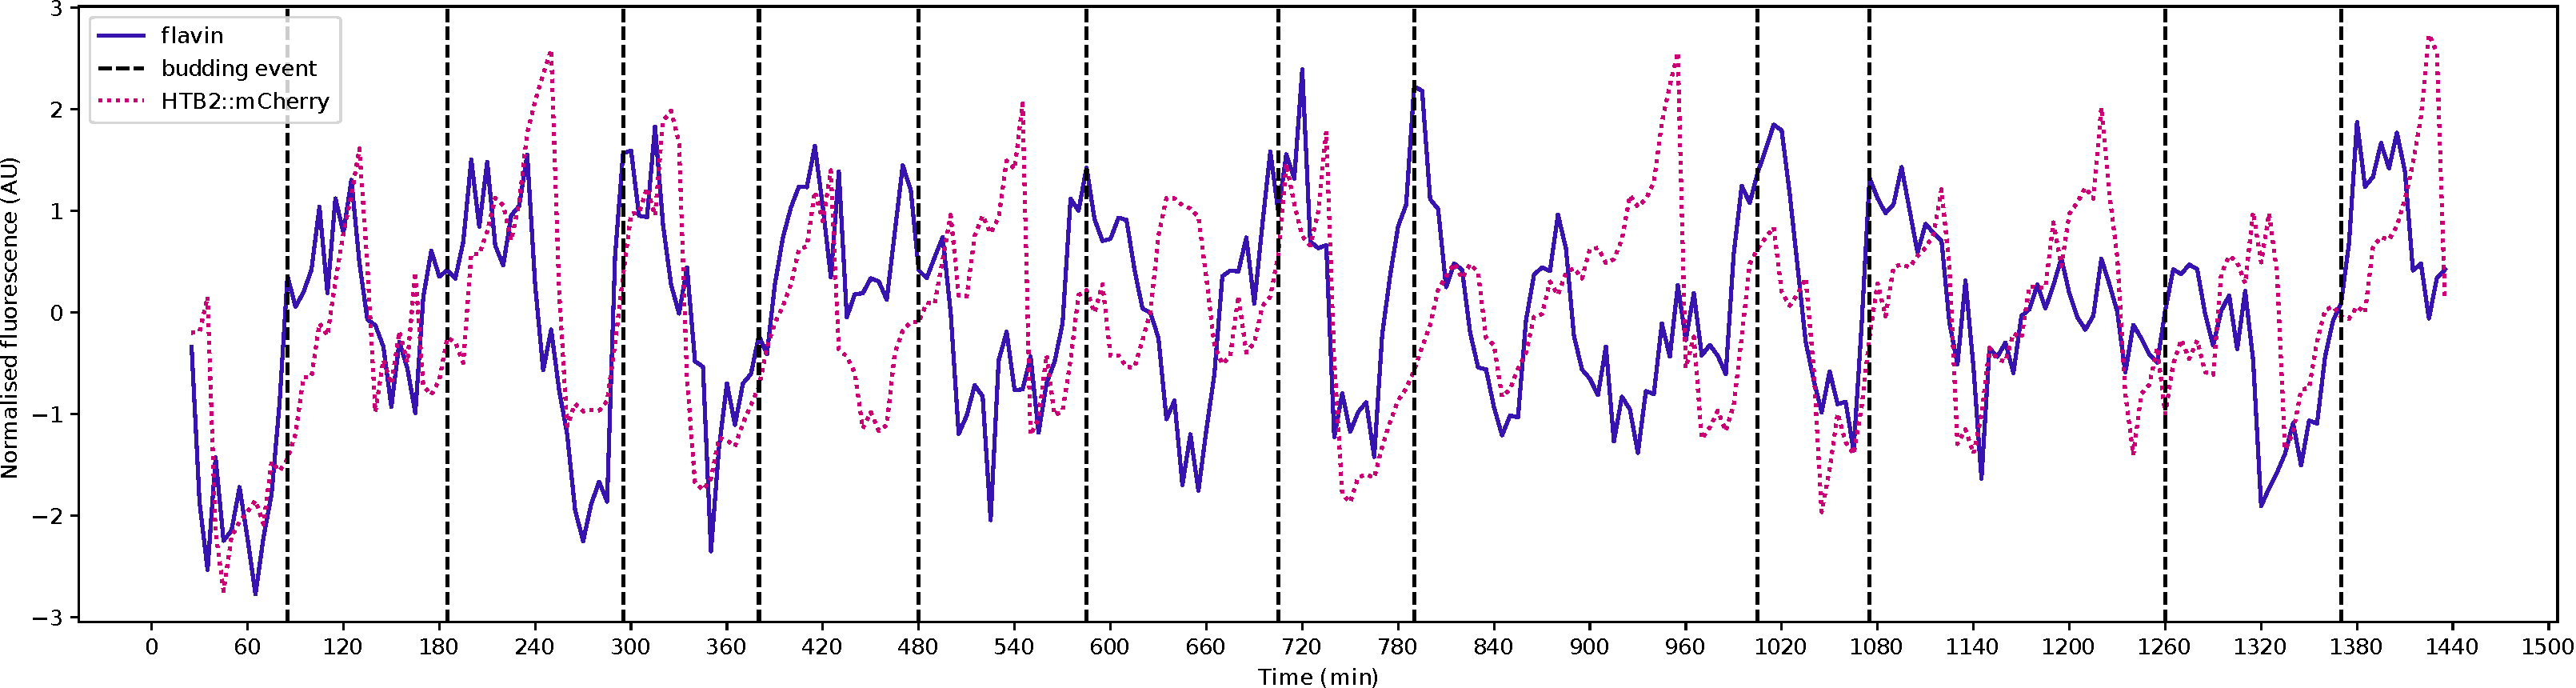
\includegraphics[width=1.0\linewidth]{single_birth_plot_edit.pdf}
    \caption[
      Flavin fluorescence and histone 2B levels in a single, representative FY4 HTB2::mCherry cell grown in \SI{20}{\gram~\litre^{-1}} glucose.
    ]{
      Flavin fluorescence (blue, solid lines) and histone 2B (orange, dotted lines) levels in a single, representative FY4 HTB2::mCherry cell grown in \SI{20}{\gram~\litre^{-1}} glucose.
      Vertical lines (black, dashed) indicate budding events.
      Star ($\star$) indicates a flavin oscillation without a corresponding cell division cycle.
    }
  \label{fig:biology-highglc-single}
\end{figure}

The HTB2::mCherry insertion allows monitoring phases of the cell division cycle through quantifying the intensity of the fluorescence of the inserted protein over time \parencite{garmendia-torresMultipleInputsEnsure2018} (Fig.\ \ref{fig:biology-htb2}), while also allowing monitoring flavin fluorescence by avoiding the overlap of flavin and GFP emission spectra.

\begin{figure}
  \centering
    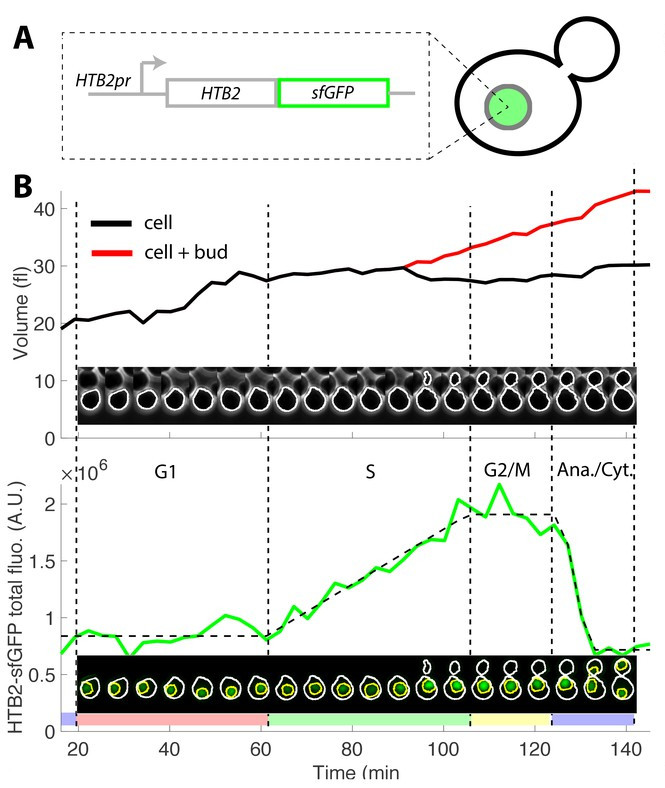
\includegraphics[width=0.5\linewidth]{garmendia-torresMultipleInputsEnsure2018_1_adapted.jpg}
    \caption[
      Engineering a fluorescent protein cassette fused to \textit{HTB2} allows the identification of phases of the cell division cycle through monitoring changes in fluorescence of the fluorescent protein.
    ]{
      \textbf{(A)} Engineering a fluorescent protein cassette fused to \textit{HTB2} \textbf{(B)} allows the identification of phases of the cell division cycle through monitoring changes in fluorescence of the fluorescent protein.
      Adapted from \textcite{garmendia-torresMultipleInputsEnsure2018}.
    }
  \label{fig:biology-htb2}
\end{figure}

Fig.\ \ref{fig:biology-highglc-single} also shows that in some cases, a metabolic oscillation occurred without cell division cycle progression or bud formation.
Such cases, also revealed by \textcite{papagiannakisAutonomousMetabolicOscillations2017} via cycles of NAD(P)H fluorescence, confirmed that the metabolic cycle is generated autonomously from the cell division cycle.

As observed, oxidation of flavin upon budding was expected for these reasons:
\begin{enumerate}
  \item Flavin fluorescence peaks (becomes most oxidised) and NAD(P)H fluorescence peaks (becomes most reduced) at the same time in chemostat cultures \parencite{murrayRedoxRegulationRespiring2011}.
  \item NAD(P)H is in the reduced form when buds form \parencite{papagiannakisAutonomousMetabolicOscillations2017}.
  \item The flavoprotein lipoamide dehydrogenase, coded by the gene \textit{LPD1}, is in redox equilibrium with NAD(P)H \parencite{sianoNADHFlavinFluorescence1989}.
\end{enumerate}

To quantify the period of the oscillators, I combined time series analysis methods.
Fig.\ \ref{fig:biology-highglc-sync-spectral} shows that flavin fluorescence oscillated at a period of approximately \SI{90}{\minute}, based on the mean Fourier spectrum and median autocorrelation function.
Figs.\ \ref{fig:biology-highglc-sync-acf} and~\ref{fig:biology-highglc-sync-acf-2} additionally show that the cell division cycle proceeded at the same period, as evidenced by the autocorrelation function of mCherry.
The duration of the cell division cycles agrees with previously reported values \parencite{herskowitzLifeCycleBudding1988}.

\begin{figure}[b!]
  \centering
  \begin{subfigure}[htpb]{0.45\textwidth}
   \centering
   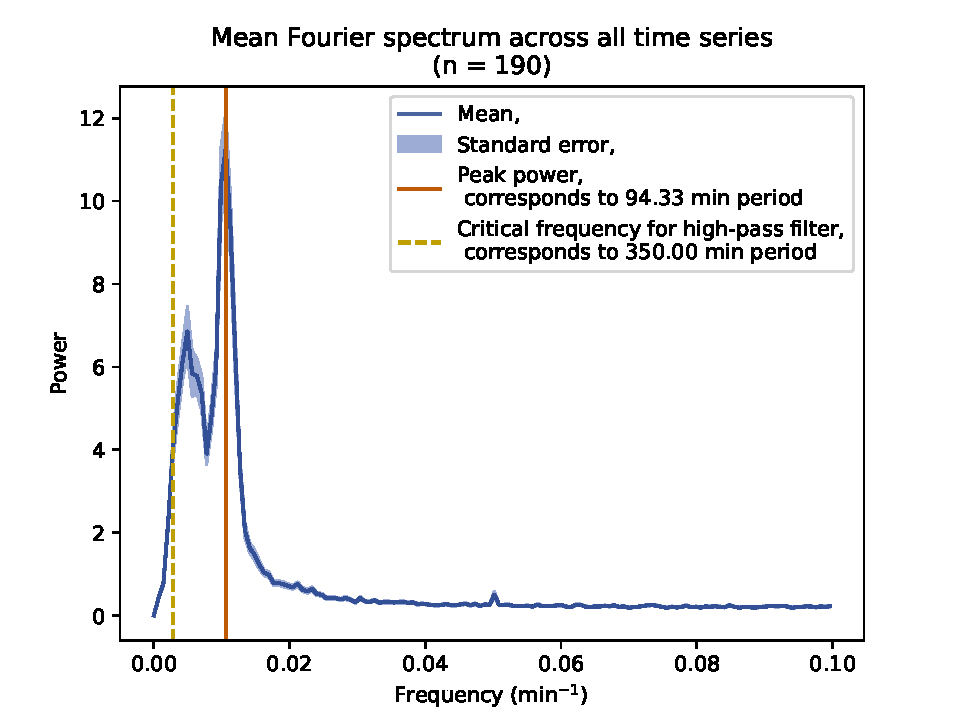
\includegraphics[width=\textwidth]{htb2mCherry_26643_14}
   \caption{
   }
   \label{fig:biology-highglc-sync-fourier}
  \end{subfigure}%
  \begin{subfigure}[htpb]{0.45\textwidth}
   \centering
   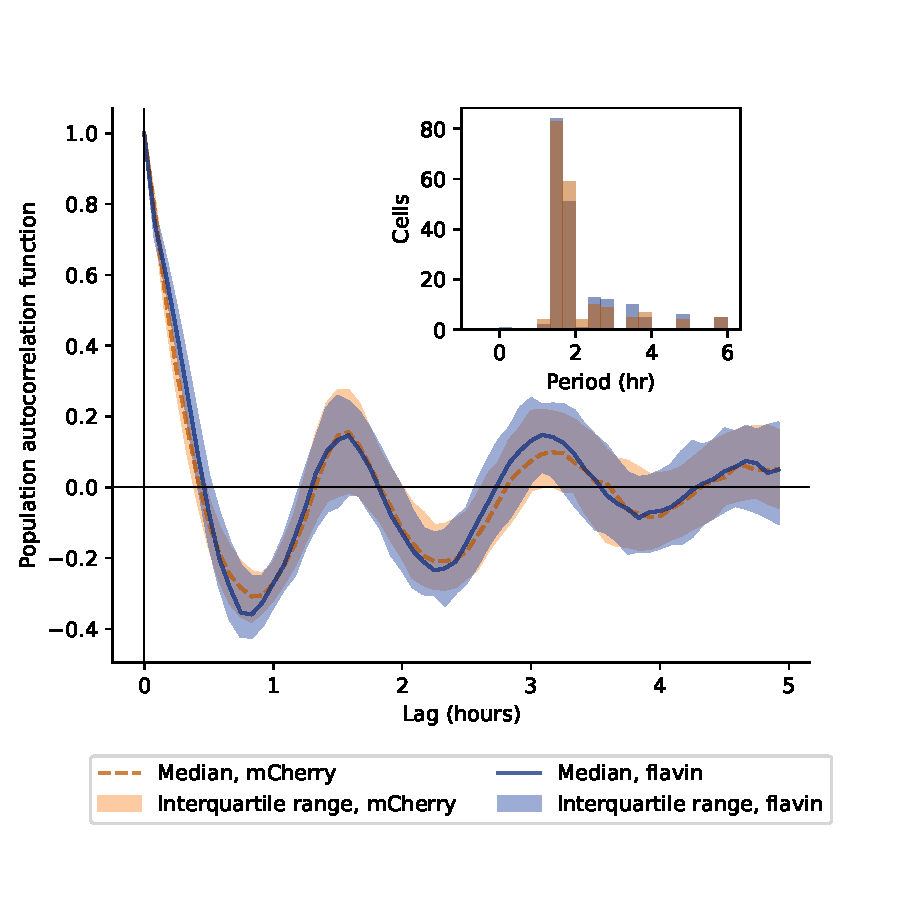
\includegraphics[width=\textwidth]{htb2mCherry_26643_12}
   \caption{
   }
   \label{fig:biology-highglc-sync-acf}
  \end{subfigure}

  \begin{subfigure}[htpb]{0.45\textwidth}
   \centering
   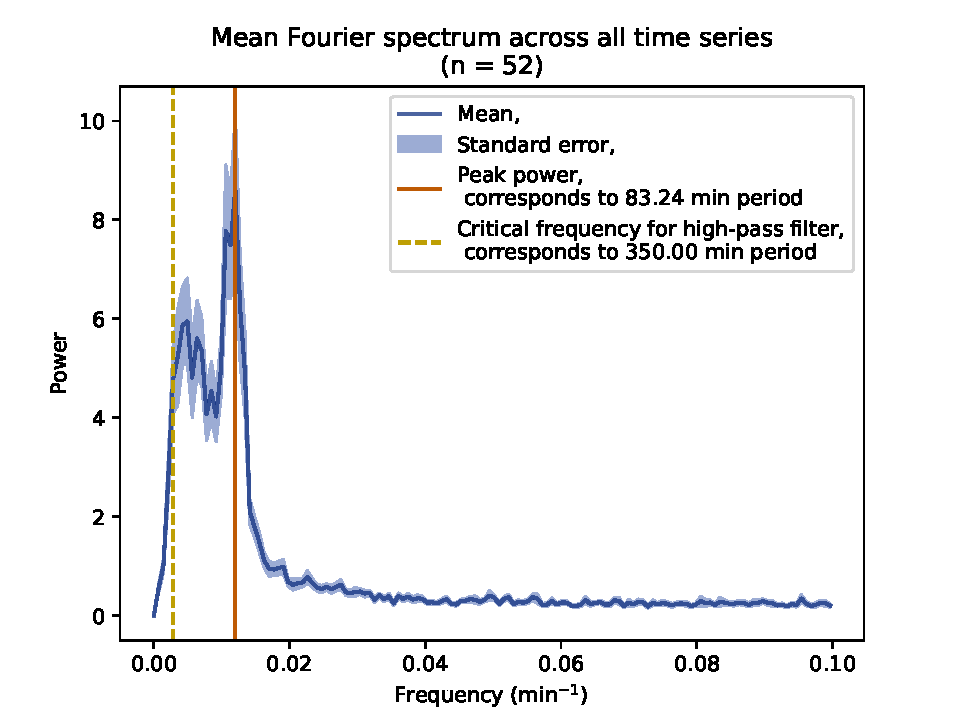
\includegraphics[width=\textwidth]{htb2mCherry_27917_14}
   \caption{
   }
   \label{fig:biology-highglc-sync-fourier-2}
  \end{subfigure}%
  \begin{subfigure}[htpb]{0.45\textwidth}
   \centering
   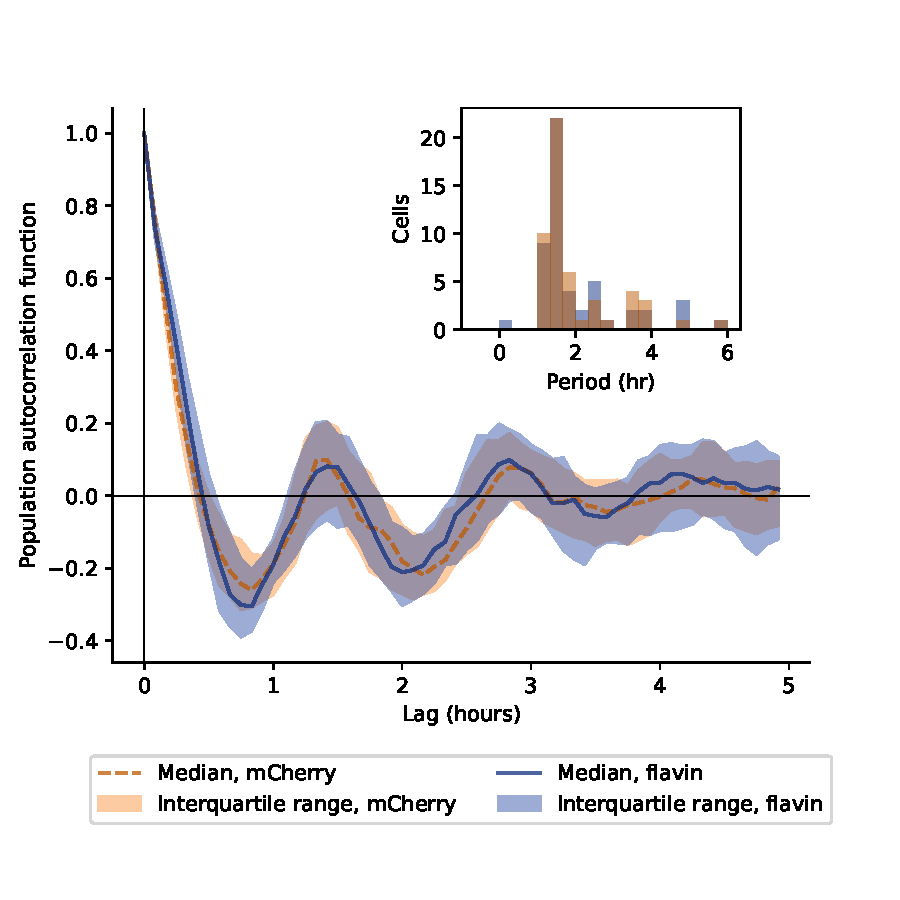
\includegraphics[width=\textwidth]{htb2mCherry_27917_12}
   \caption{
   }
   \label{fig:biology-highglc-sync-acf-2}
  \end{subfigure}

  \caption[
    Mean Fourier spectrum of flavin fluorescence time series across cells.
    Median autocorrelation functions of flavin fluorescence and histone 2B levels time series, along with the periods of each oscillator across cells.
    Data are from FY4 HTB2::mCherry cells under \SI{20}{\gram~\litre^{-1}} glucose.
  ]{
    \textbf{(\ref{fig:biology-highglc-sync-fourier},~\ref{fig:biology-highglc-sync-fourier-2})} Mean Fourier spectrum of flavin fluorescence time series across cells. \textbf{(\ref{fig:biology-highglc-sync-acf},~\ref{fig:biology-highglc-sync-acf-2})} Median autocorrelation functions of flavin fluorescence (blue) and histone 2B levels (orange) time series, along with \textit{\textbf{(insets)}} the periods of each oscillator across cells as determined by the frequency with the greatest power in each signal's Fourier spectrum.
    Data are from FY4 HTB2::mCherry cells under \SI{20}{\gram~\litre^{-1}} glucose; two experiment repeats shown.
  }
  \label{fig:biology-highglc-sync-spectral}
\end{figure}

To visualise the relationship between the metabolic cycle and the cell division cycle,
Fig.\ \ref{fig:biology-highglc-sync-corr} shows that
budding events synchronise with peaks in fluorescence and
that the cell division cycle varies between cells,
with most just under \SI{2}{\hour}, agreeing with Fig.\ \ref{fig:biology-highglc-sync-acf} (inset).
The oscillatory shape of the median flavin fluorescence time series when aligned to the first budding event (Fig.\ \ref{fig:biology-highglc-sync-median}) further confirms the synchrony between the metabolic cycle and budding events.

\begin{figure}[p]
  \centering
  \begin{subfigure}[htpb]{0.45\textwidth}
   \centering
   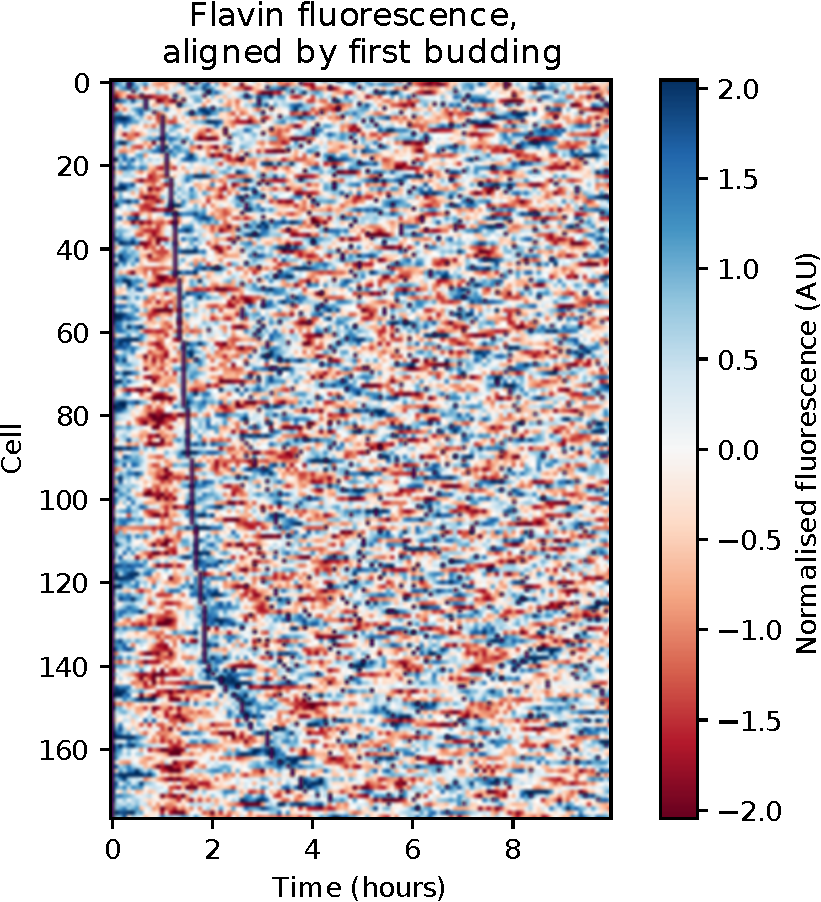
\includegraphics[width=\textwidth]{heatmap_edit.pdf}
   \caption{
   }
   \label{fig:biology-highglc-sync-heatmap}
  \end{subfigure}%
  \begin{subfigure}[htpb]{0.45\textwidth}
   \centering
   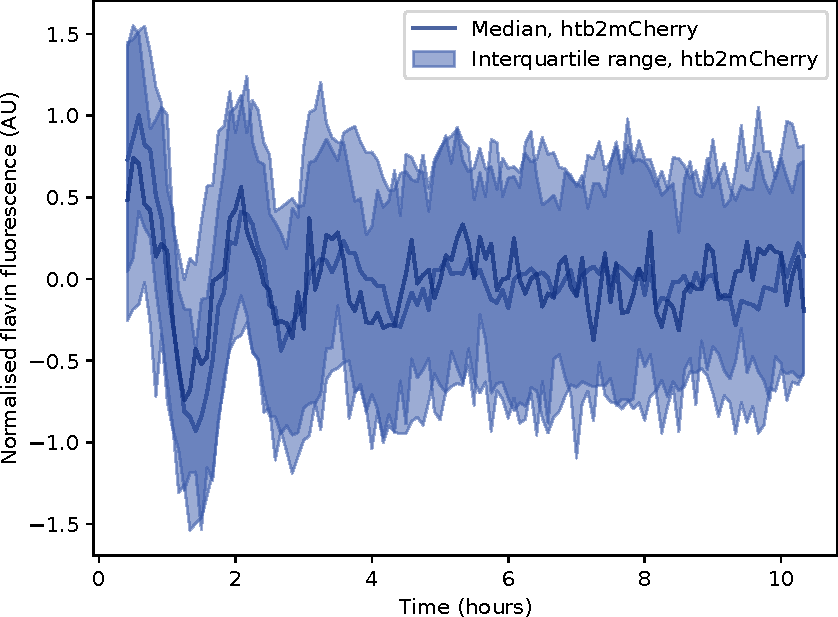
\includegraphics[width=\textwidth]{htb2mCherry_highglcreps_6.pdf}
   \caption{
   }
   \label{fig:biology-highglc-sync-median}
  \end{subfigure}

  \begin{subfigure}[htpb]{0.7\textwidth}
   \centering
   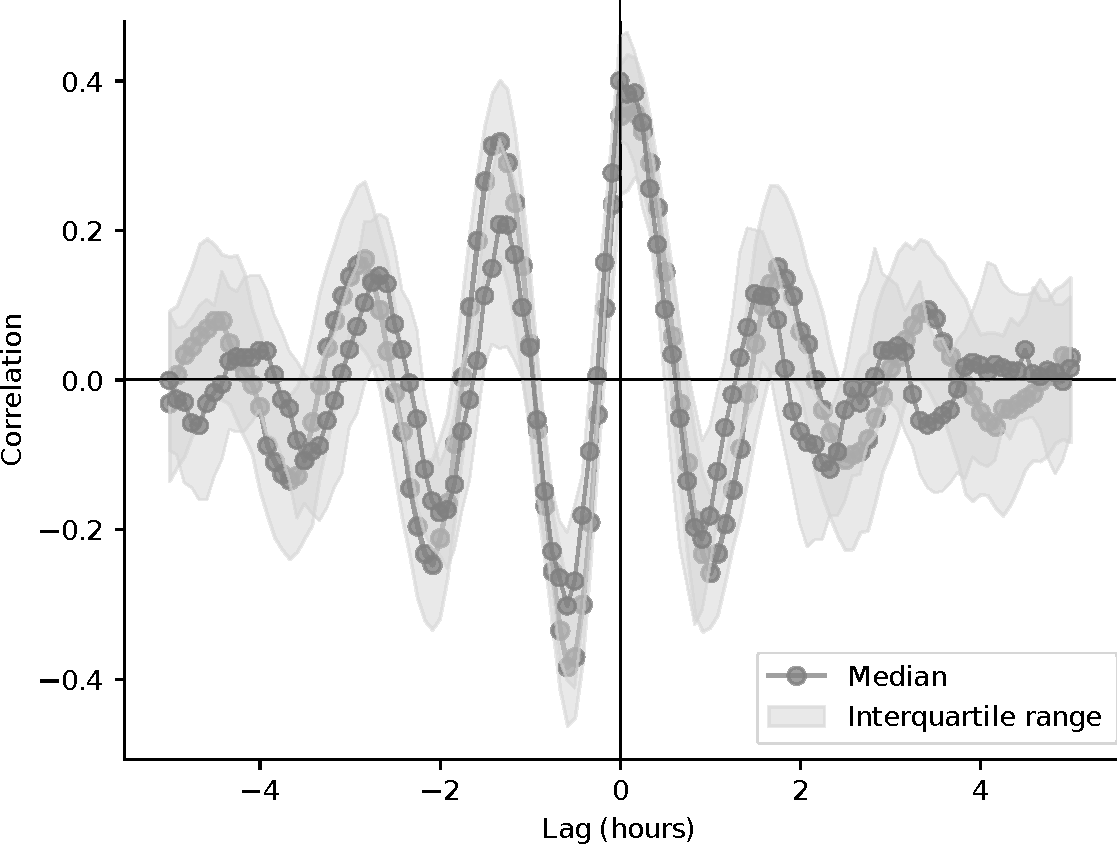
\includegraphics[width=\textwidth]{xcf_highglcreps.pdf}
   \caption{
   }
   \label{fig:biology-highglc-sync-xcf}
  \end{subfigure}

  \caption[
    Heatmap showing the flavin fluorescence and budding events of each cell over time.
    Median flavin fluorescence signal across cells, aligned to first budding event.
    Median cross-correlation function between flavin and histone 2B signals.
    Data are from FY4 HTB2::mCherry cells in \SI{20}{\gram~\litre^{-1}} glucose.
  ]{
    \textbf{(\ref{fig:biology-highglc-sync-heatmap})}
    Heatmap showing the flavin fluorescence (pixels on a red-blue scale) and budding events (black pixels) of each cell over time.
    Signals are aligned by the first budding event.
    \textbf{(\ref{fig:biology-highglc-sync-median})}
    Median flavin fluorescence signal across cells, aligned to first budding event (two repeats: $n_{1}=361$, $n_{2}=144$).
    \textbf{(\ref{fig:biology-highglc-sync-xcf})}
    Median cross-correlation function between flavin and histone 2B signals (two repeats: $n_{1}=392$, $n_{2}=170$).
    Data are from FY4 HTB2::mCherry cells in \SI{20}{\gram~\litre^{-1}} glucose.
  }
  \label{fig:biology-highglc-sync-corr}
\end{figure}

Finally, to quantify the relationship between the metabolic cycle and the cell division cycle, I computed the cross-correlation function between the flavin and mCherry signals across the population (Fig.\ \ref{fig:biology-highglc-sync-xcf}).
The flavin signal peaks, on average, precede the mCherry signal peaks by \SI{5}{\minute}, as evidenced by the location of the peak of the cross-correlation function that is closest to the vertical axis.
The cross-correlation function thus demonstrates the coincidence between peaks of flavin oscillations and mitosis.


%\section[Abrupt nutrient changes]{Cells autonomously generate flavin oscillations, independently of the cell division cycle, in response to abrupt nutrient changes.}
\section{Decoupling between the metabolic and cell division cycles}
\label{sec:biology-abrupt}


To provide additional evidence that cells generate metabolic oscillations autonomously of the cell division cycle, I created a condition in which cells did not undergo cell division.
Specifically, I did so by inducing starvation: I cultured FY4 and HTB2::mCherry cells in \SI{7.5}{\gram~\litre^{-1}} glucose for \SI{7}{\hour}, switching them to \SI{0}{\gram~\litre^{-1}} glucose for \SI{8}{\hour}, and then resumed \SI{7.5}{\gram~\litre^{-1}} glucose for \SI{7}{\hour}.
This abrupt induction of starvation is similar to experiments described by \textcite{bagameryPutativeBetHedgingStrategy2020}, which showed that a population of genetically identical budding yeast cells, upon glucose starvation, formed two sub-populations that had different cellular physiology.

Fig.\ \ref{fig:biology-starvation} shows that when cells were in high glucose, metabolic oscillations were asynchronous, consistent with Section~\ref{sec:biology-sync}, \textcite{papagiannakisAutonomousMetabolicOscillations2017}, and \textcite{baumgartnerFlavinbasedMetabolicCycles2018}.
When cells grown in high glucose were abruptly starved of glucose, their flavin oscillations reset their phase.

\begin{figure}
  \centering
  \begin{subfigure}[htpb]{1.0\textwidth}
   \centering
   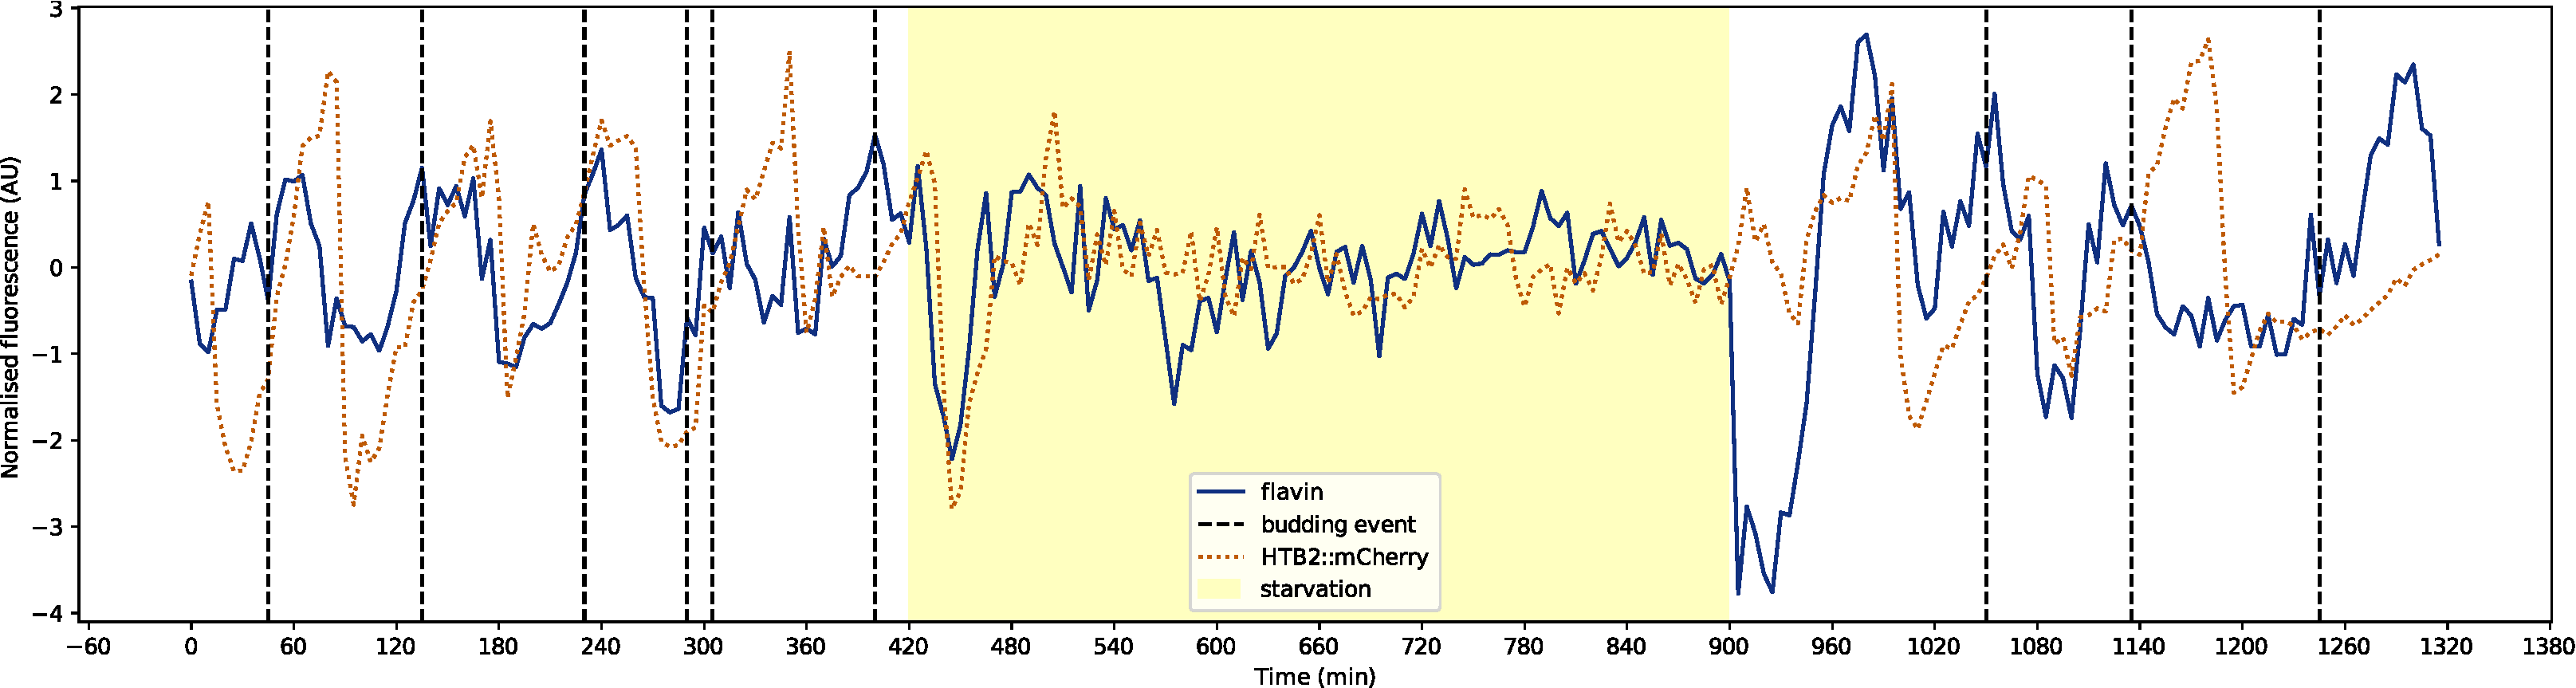
\includegraphics[width=\textwidth]{starvation_single_birth_plot_new_edit.pdf}
   \caption{
   }
   \label{fig:biology-starvation-single}
  \end{subfigure}

  \begin{subfigure}[htpb]{0.9\textwidth}
   \centering
   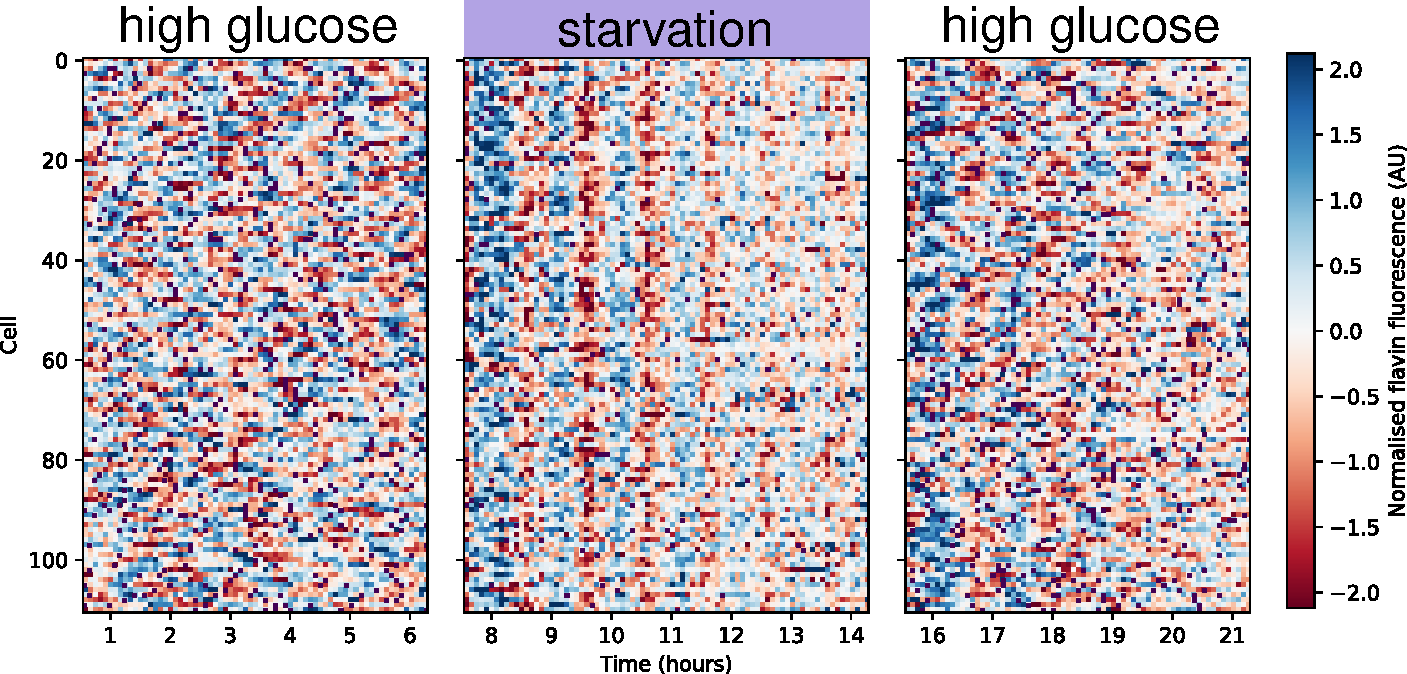
\includegraphics[width=\textwidth]{heatmap_012_edit.pdf}
   \caption{
   }
   \label{fig:biology-starvation-heatmap}
  \end{subfigure}

  \caption[
    Flavin fluorescence and histone 2B levels in a single, representative FY4 HTB2::mCherry cell.
    Heatmap showing the flavin fluorescence and budding events of each cell.
    Data are from FY4 and HTB2::mCherry cells, subject to glucose starvation.
  ]{
    \textbf{(\ref{fig:biology-starvation-single})}
    Flavin fluorescence (blue, solid lines) and histone 2B (orange, dotted lines) levels in a single, representative FY4 HTB2::mCherry cell.
    Vertical lines (black, dashed) indicate budding events.
    Shading (yellow) indicates glucose starvation.
    \textbf{(\ref{fig:biology-starvation-heatmap})}
    Heatmap showing the flavin fluorescence (pixels on a red-blue scale) and budding events (black pixels) of each cell.
    Data are from FY4 and HTB2::mCherry cells, subject to \SI{7.5}{\gram~\litre^{-1}} glucose for \SI{7}{\hour} before being abruptly switched to \SI{0}{\gram~\litre^{-1}} glucose for \SI{8}{\hour} and then resumed to \SI{7.5}{\gram~\litre^{-1}} glucose for \SI{7}{\hour}.
  }
  \label{fig:biology-starvation}
\end{figure}

Fig.\ \ref{fig:biology-starvation-gr-budprob} further shows that during starvation, these flavin oscillations continued, while growth rate dropped and budding events were sparse.
The partial, rather than full, recovery of growth rate after starvation may be explained by accumulated phototoxicity over the course of the experiment generated by fluorescence imaging, with similar patterns across all experiments.
Alternatively, the partial recovery of growth rate could also be explained by memory of glucose starvation.
In addition, the lower cumulative number of budding events in the HTB2::mCherry strain, consistent across all experiments, may be explained by the increased phototoxicity generated by mCherry imaging in five z-slices (Methods Section~\ref{subsec:methods-microfluidics}).

\begin{figure}
  \centering
  \begin{subfigure}[htpb]{0.45\textwidth}
   \centering
   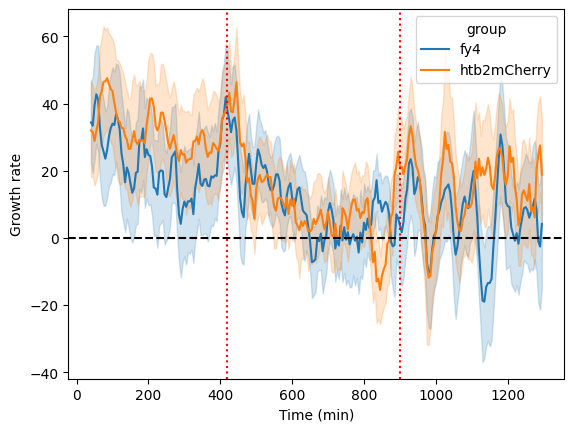
\includegraphics[width=\textwidth]{allstrains_19972_gr}
   \caption{
   }
   \label{fig:biology-starvation-gr}
  \end{subfigure}%
  \begin{subfigure}[htpb]{0.45\textwidth}
   \centering
   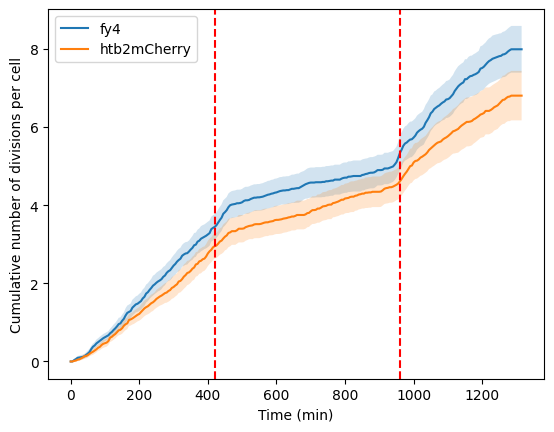
\includegraphics[width=\textwidth]{allstrains_19972_cumul}
   \caption{
   }
   \label{fig:biology-starvation-cumul}
  \end{subfigure}

  \caption[
    Mean growth rate, derived from changes in the sum of estimated parent cell and bud volumes and
    mean cumulative number of budding events per cell
    of FY4 and HTB2::mCherry strains over time during the glucose-starvation experiment.
  ]{
    \textbf{(\ref{fig:biology-starvation-gr})}
    Mean growth rate, derived from changes in the sum of estimated parent cell and bud volumes (shading: 95\% confidence intervals) and
    \textbf{(\ref{fig:biology-starvation-cumul})}
    mean cumulative number of budding events per cell (shading: confidence intervals from bootstrapping, $n=30$)
    of FY4 (blue) and HTB2::mCherry (orange) strains over time during the glucose-starvation experiment.
    Vertical lines (red) show changes in the nutrient medium.
  }
  \label{fig:biology-starvation-gr-budprob}
\end{figure}

% Does this paragraph belong in the discussion?
The results show that metabolic oscillations can be generated when the cell division cycle is halted, providing strong evidence that the metabolic cycle is generated autonomously and independently of the cell division cycle.
In addition, the results show that each cell can individually reset the phase of its metabolic cycle in response to abrupt changes in environmental conditions.
Similar phenomena have been observed upon bulk addition of carbon sources \parencite{kuangMsn2RegulateExpression2017, krishnaMinimalPushPull2018}.
Importantly, the results suggest that diffusion of signalling chemicals between cells is not required for generation of metabolic cycles.
Combined with results from the previous section, my data suggest that the metabolic cycle responds to external conditions and create windows of opportunity for initiating the cell division cycle, if conditions are favourable for growth.

The model in which the metabolic cycle creates windows of opportunity for the cell division cycle implies that, upon starvation, cell division cycles progress to the next gap phase (G\textsubscript{1} or G\textsubscript{2}/M) while the metabolic cycle continues.
To test this implication, Fig.\ \ref{fig:biology-starvation-raw} shows that cells may remain in G\textsubscript{1} (Fig.\ \ref{fig:biology-starvation-raw-2}), as evidenced by low mCherry intensity, or in G\textsubscript{2}/M (Fig.\ \ref{fig:biology-starvation-raw-1}), as evidenced by high mCherry intensity.

\begin{figure}[hb!]
  \centering
  \begin{subfigure}[htpb]{1.0\textwidth}
   \centering
   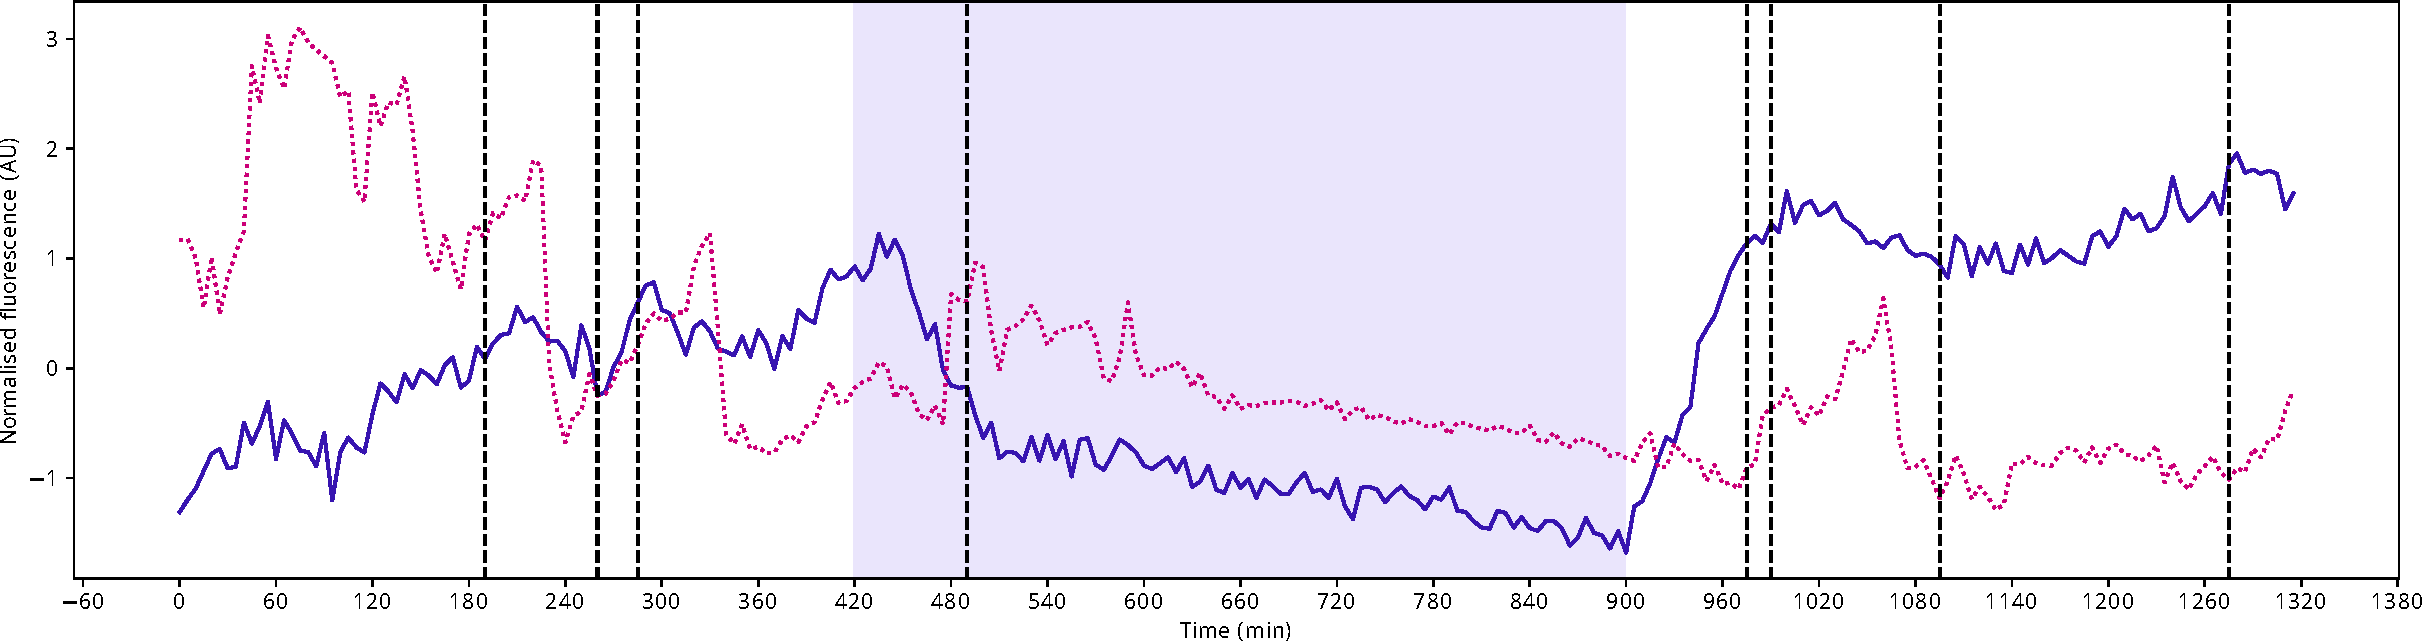
\includegraphics[width=\textwidth]{starvation_raw_13-39-01.pdf}
   \caption{
   }
   \label{fig:biology-starvation-raw-2}
  \end{subfigure}

  \begin{subfigure}[htpb]{1.0\textwidth}
   \centering
   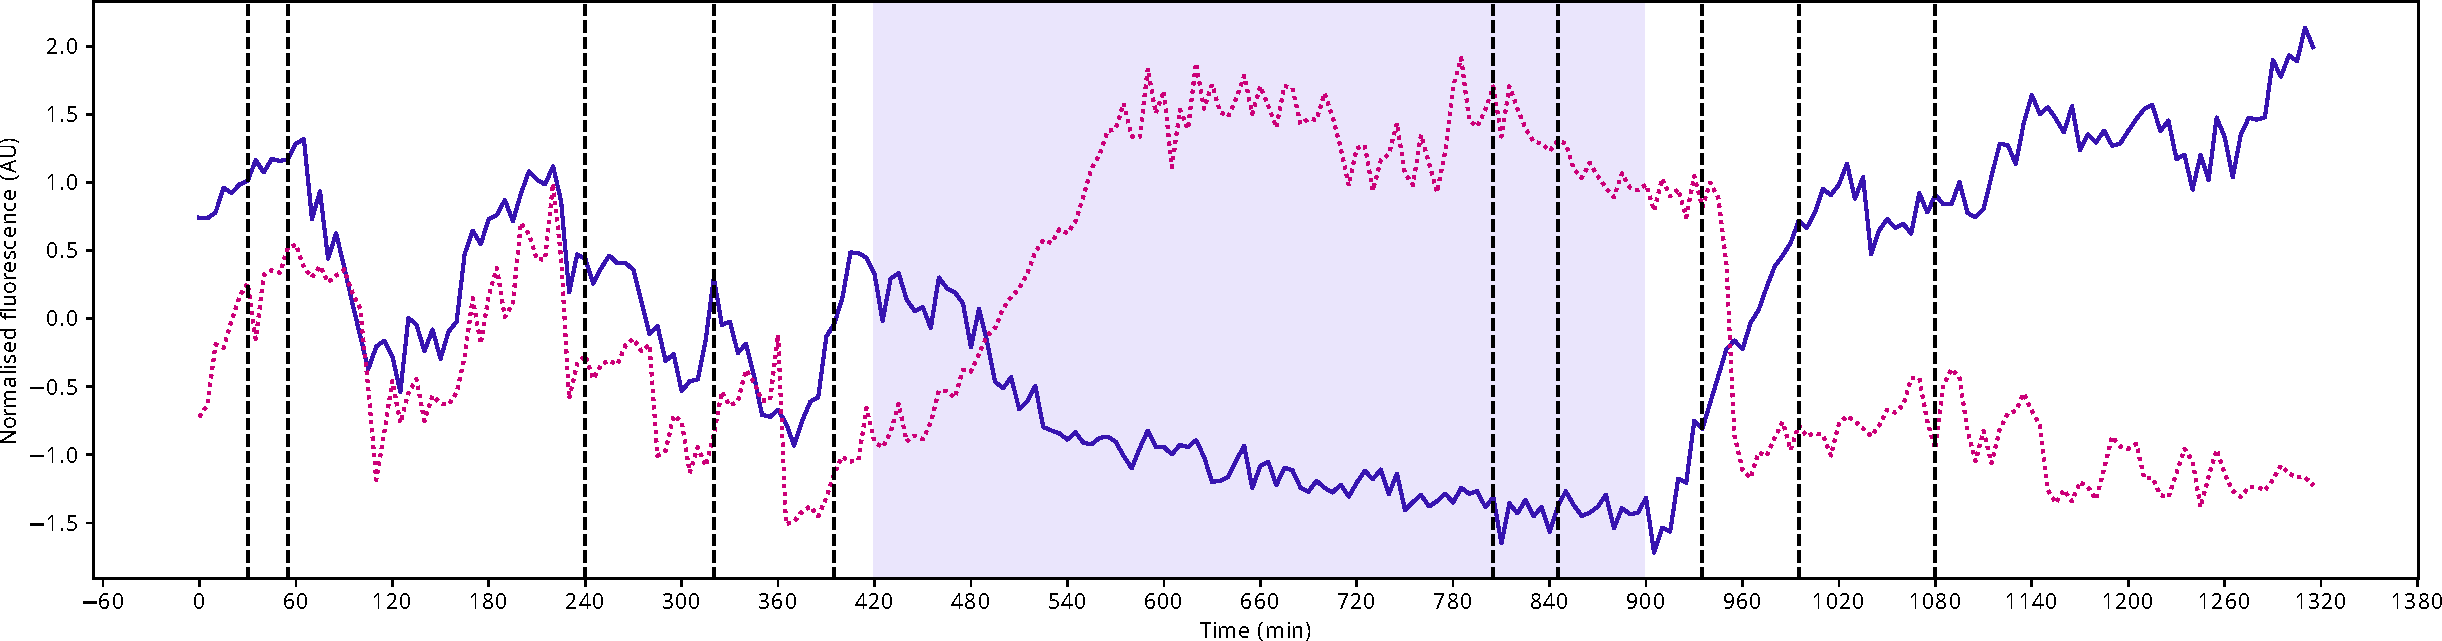
\includegraphics[width=\textwidth]{starvation_raw_13-07-02.pdf}
   \caption{
   }
   \label{fig:biology-starvation-raw-1}
  \end{subfigure}

  \caption[
    Flavin fluorescence and histone 2B levels in two sample FY4 HTB2::mCherry cells in the glucose starvation experiment.
  ]{
    Flavin fluorescence (blue, solid lines) and histone 2B (orange, dotted lines) levels in two sample FY4 HTB2::mCherry cells in the glucose starvation experiment.
    Vertical lines (black, dashed) indicates budding events.
    Shading (yellow) indicate glucose starvation.
    \textbf{(\ref{fig:biology-starvation-raw-2})} is an example of a cell with a low intensity of mCherry during starvation, while \textbf{(\ref{fig:biology-starvation-raw-1})} is an example with a high intensity of mCherry.
    %Unlike other figures,
    The flavin and mCherry time series were normalised to give a mean of 0 and standard deviation of 1 so that they can be plotted on the same vertical axes, but the high-pass Butterworth filter was not applied.
  }
  \label{fig:biology-starvation-raw}
\end{figure}

Extending this investigation across a population of cells, Fig.\ \ref{fig:biology-starvation-histogram-mCherry} shows that the distribution of mCherry intensity becomes broader during starvation before resuming to a distribution resembling the initial condition upon restoration of glucose.
This observation can be explained by a larger proportion of cells in G\textsubscript{2}/M, giving high mCherry intensity, in contrast to the usually short time cells spend in G\textsubscript{2}/M relative to the rest of the cell division cycle (Fig.\ \ref{fig:biology-htb2}).
In contrast, Fig.\ \ref{fig:biology-starvation-histogram-flavin} suggests that during starvation, the distribution of flavin intensity became narrower.
% WHAT THE HECK DID I WRITE HERE??  I DON'T UNDERSTAND WHY I WROTE THIS.
%This observation can be explained by lower-amplitude oscillations during starvation, which was evidenced by a lower signal-to-noise ratio ($\bar{x}_{\mathrm{before}} = 2.86$, $\bar{x}_{\mathrm{starvation}} = 2.17$, $\bar{x}_{\mathrm{after}} = 4.09$; two-sided Kolmogorov-Smirnov test: starvation vs before $p = \num{6.9e-15}$, starvation vs after $p = \num{6.6d-18}$).
In addition, the overall higher intensity of flavin signals after starvation compared to before starvation suggest some memory of starvation.

\begin{figure}
  \centering
  \begin{subfigure}[htpb]{0.5\textwidth}
   \centering
   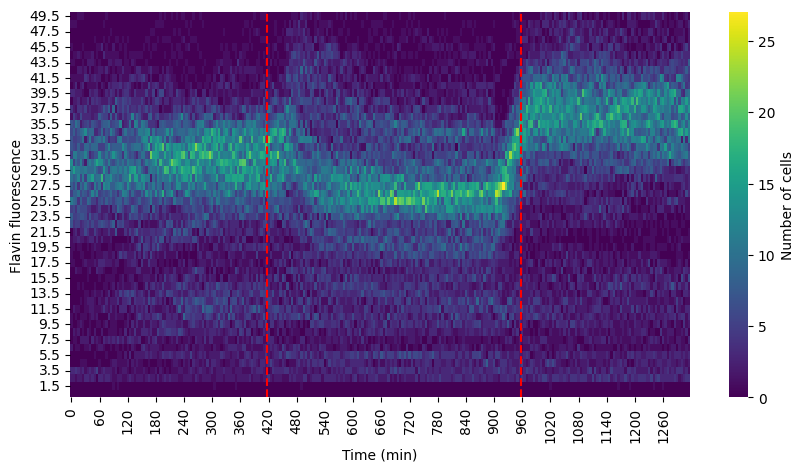
\includegraphics[width=\textwidth]{19972_distribs_flavin.png}
   \caption{
   }
   \label{fig:biology-starvation-histogram-flavin}
  \end{subfigure}%
  \begin{subfigure}[htpb]{0.5\textwidth}
   \centering
   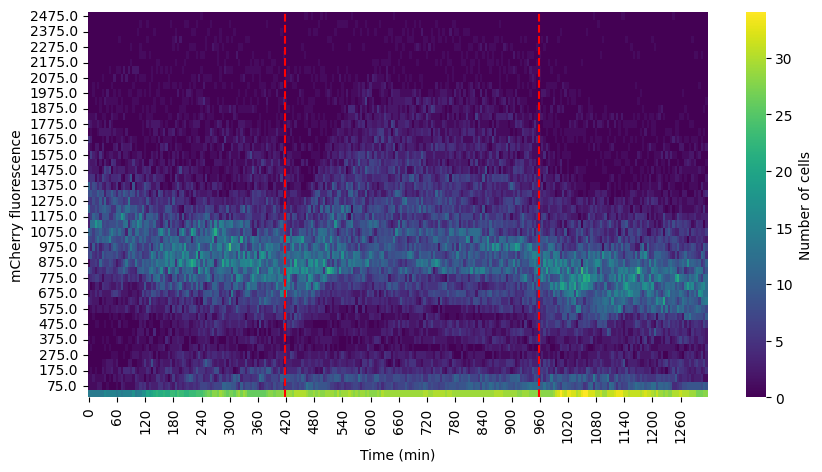
\includegraphics[width=\textwidth]{19972_distribs_mCherry.png}
   \caption{
   }
   \label{fig:biology-starvation-histogram-mCherry}
  \end{subfigure}

  \begin{subfigure}[htpb]{0.5\textwidth}
   \centering
   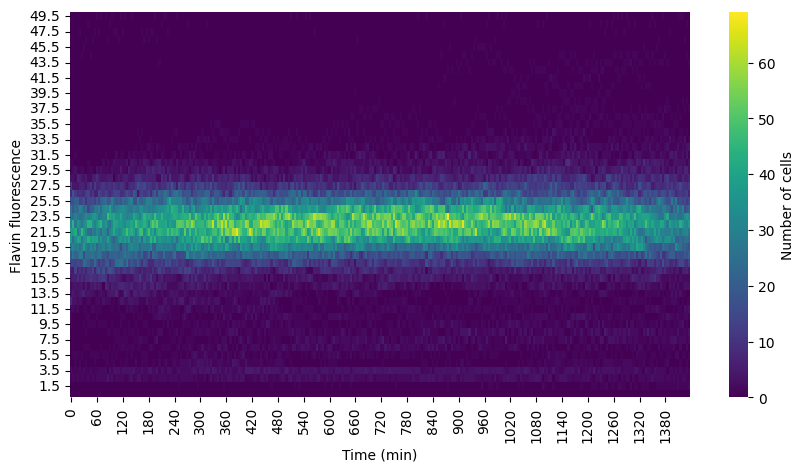
\includegraphics[width=\textwidth]{26643_distribs_flavin.png}
   \caption{
   }
   \label{fig:biology-highglc-histogram-flavin}
  \end{subfigure}%
  \begin{subfigure}[htpb]{0.5\textwidth}
   \centering
   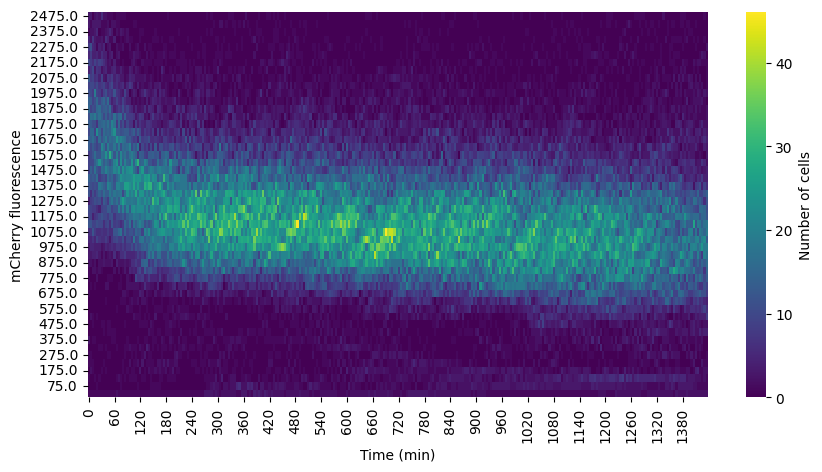
\includegraphics[width=\textwidth]{26643_distribs_mCherry.png}
   \caption{
   }
   \label{fig:biology-highglc-histogram-mCherry}
  \end{subfigure}

  \caption[
    Distributions of flavin and mCherry fluorescence over time, for the glucose-starvation experiment.
  ]{
    Distributions of \textbf{(\ref{fig:biology-starvation-histogram-flavin})} flavin and \textbf{(\ref{fig:biology-starvation-histogram-mCherry})} mCherry fluorescence over time, for the glucose-starvation experiment.
    Vertical lines (red, dashed), indicate times of medium changes.
    As a control, distributions of \textbf{(\ref{fig:biology-highglc-histogram-flavin})} flavin and \textbf{(\ref{fig:biology-highglc-histogram-mCherry})} mCherry fluorescence over time for the high glucose (\SI{20}{\gram~\litre^{-1}}) experiment are also shown.
    Raw time series were used to calculate the distributions.
  }
  \label{fig:biology-starvation-histogram}
\end{figure}


\section{Metabolic cycles in different genetic backgrounds}
\label{sec:biology-backgrounds}

To show that the metabolic cycle is robust,
I monitored flavin autofluorescence signals from the auxotrophic BY4741 strain.
Cells of this strain were grown in minimal medium supplemented with uracil and the amino acids required for this strain to grow, in addition to \SI{10}{\gram~\litre^{-1}} glucose as the carbon source.
Showing that metabolic cycles occur in an auxotroph is important because it shows that many cellular aspects must be impaired for the cycle to disappear, thus suggesting that the metabolic cycle is an intrinsic property of budding yeast.
Similar to FY4 HTB2::mCherry cells, BY4741 cells showed robust, consistent oscillations in flavin fluorescence that peak upon budding (Fig.\ \ref{fig:biology-by4741-sync}), although metabolic cycles have a period of $\approx$\SI{75}{\minute} in this case.
The shorter period may be explained by a lack of burden caused by a lack of an mCherry insertion, and by nutritional supplements.
% Discussion (probably in discussion section at the end): to be 'proper', I should perform an experiment with the BY4741 HTB2::mCherry I engineered.

\begin{figure}
  \centering
  \begin{subfigure}[htpb]{0.45\textwidth}
   \centering
   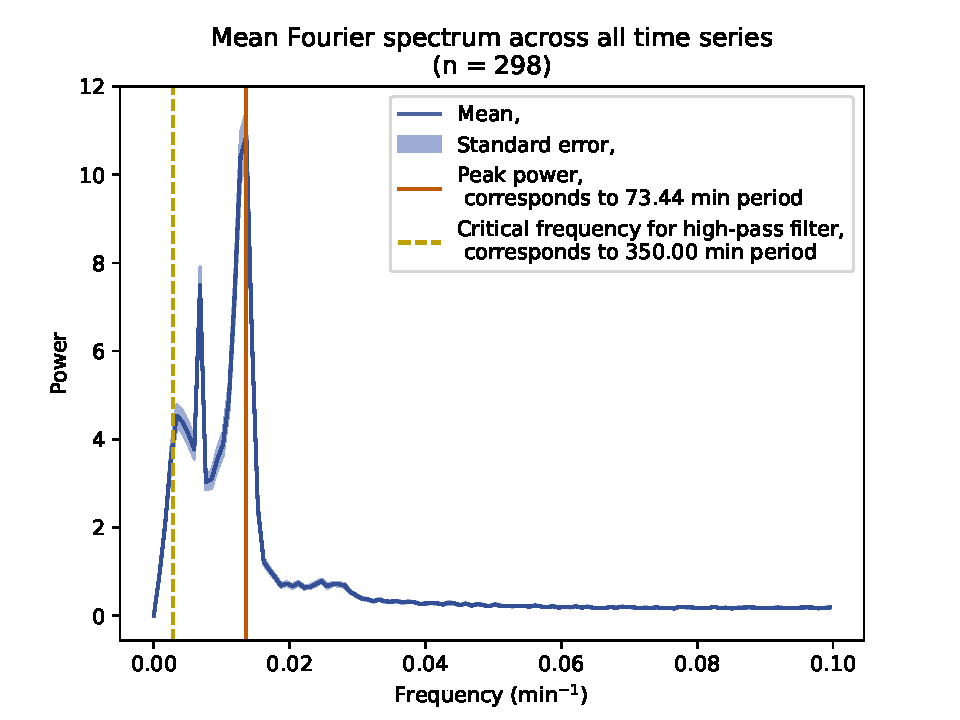
\includegraphics[width=\textwidth]{by4741_491_13}
   \caption{
   }
   \label{fig:biology-by4741-sync-fourier}
  \end{subfigure}%
  \begin{subfigure}[htpb]{0.45\textwidth}
   \centering
   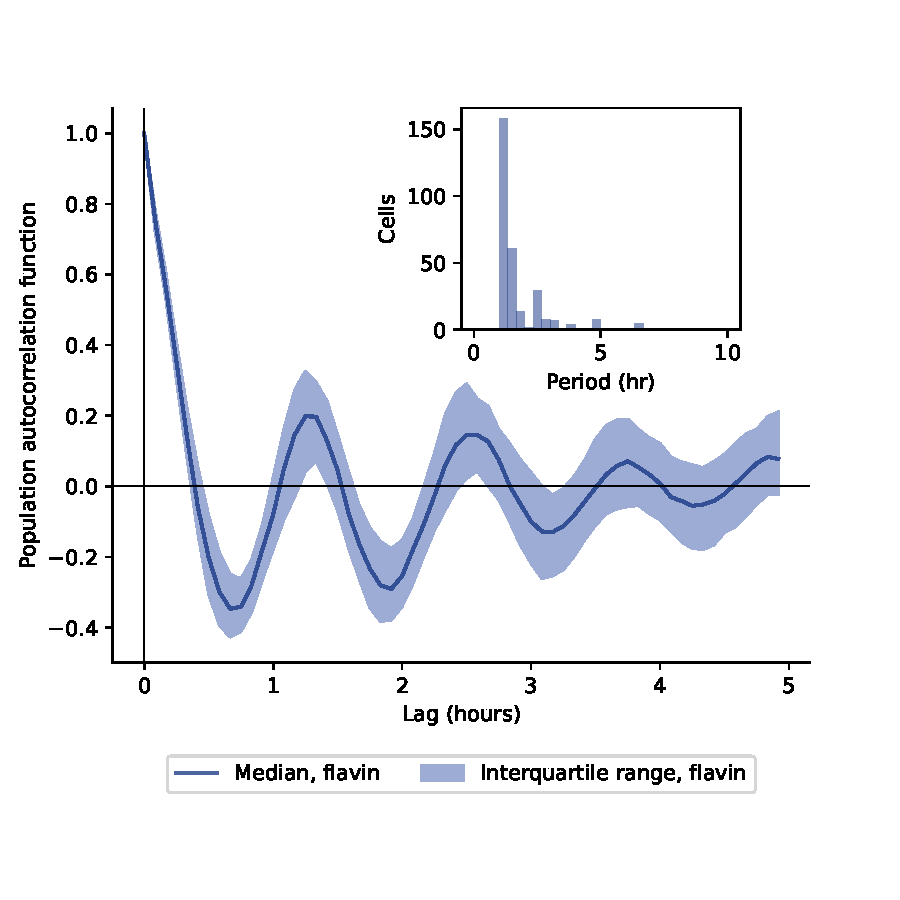
\includegraphics[width=\textwidth]{by4741_491_12}
   \caption{
   }
   \label{fig:biology-by4741-sync-acf}
  \end{subfigure}

  \begin{subfigure}[htpb]{0.45\textwidth}
   \centering
   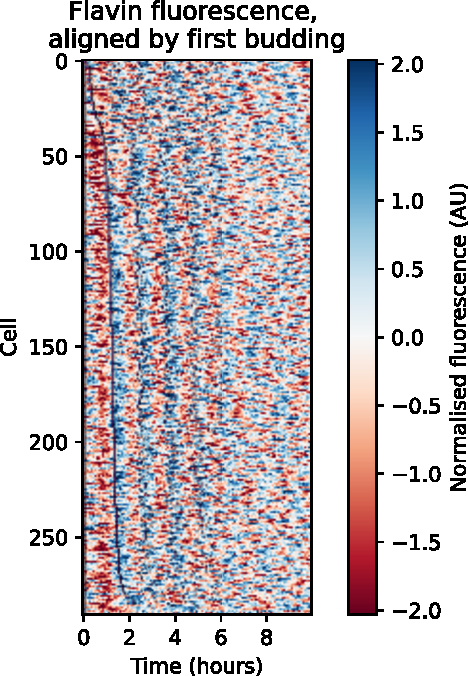
\includegraphics[width=\textwidth]{by4741_491_7.pdf}
   \caption{
   }
   \label{fig:biology-by4741-sync-heatmap}
  \end{subfigure}%
  \begin{subfigure}[htpb]{0.45\textwidth}
   \centering
   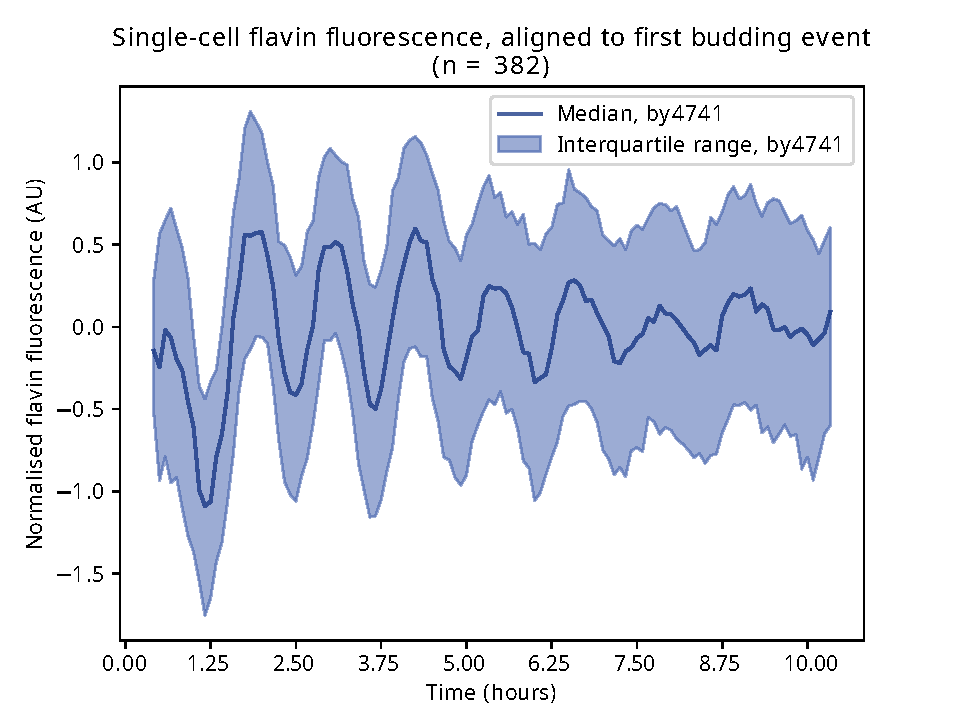
\includegraphics[width=\textwidth]{by4741_491_6}
   \caption{
   }
   \label{fig:biology-by4741-sync-median}
  \end{subfigure}

  \caption[
    Mean Fourier spectrum of flavin fluorescence time series across cells.
    Median autocorrelation function of flavin fluorescence time series, along with the periods across cells.
    Heatmap showing the flavin fluorescence and budding events of each cell.
    Median flavin fluorescence signal across cells, aligned to first budding event.
    Data are from BY4741 cells in \SI{10}{\gram~\litre^{-1}} glucose.
  ]{
    \textbf{(\ref{fig:biology-by4741-sync-fourier})} Mean Fourier spectrum of flavin fluorescence time series across cells.
    \textbf{(\ref{fig:biology-by4741-sync-acf})} Median autocorrelation function of flavin fluorescence time series, along with \textit{\textbf{(inset)}} the periods across cells as determined by the frequency with the greatest power in each signal's Fourier spectrum.
    \textbf{(\ref{fig:biology-by4741-sync-heatmap})}
    Heatmap showing the flavin fluorescence (pixels on a red-blue scale) and budding events (black pixels) of each cell.
    Signals are aligned by the first budding event.
    \textbf{(\ref{fig:biology-by4741-sync-median})}
    Median flavin fluorescence signal across cells, aligned to first budding event.
    Data are from BY4741 cells in \SI{10}{\gram~\litre^{-1}} glucose.
  }
  \label{fig:biology-by4741-sync}
\end{figure}

FY4 and BY4741 both derive from the S288c background strain.
To show that the metabolic cycle is generated from a budding yeast strain other than S288c background strains, I performed a similar experiment with the prototrophic CEN.PK strain grown in minimal medium.
Showing that metabolic cycles additionally occur in a different genetic background is important to emphasise that the cycles are intrinsic to budding yeast.
CEN.PK is an important background to consider because it harbours genetic differences relative to S288c that results in physiological differences, including biotin prototrophy and malate metabolism \parencite{nijkampNovoSequencingAssembly2012}.
Furthermore, CEN.PK has greater mitochondrial stability and a better gene regulatory response to levels of oxygen, owing to the insertion mutation that deactivates the \textit{HAP1} gene in S288c \parencite{gaisneNaturalMutationSaccharomyces1999}.
Fig.\ \ref{fig:biology-cenpk-sync} suggests that CEN.PK113-7D cells exhibited \SI{90}{\minute} flavin oscillations that were synchronised with budding events, similar to FY4 cells, thus further confirming the robustness of the metabolic cycle across genetic backgrounds.

\begin{figure}
  \centering
  \begin{subfigure}[htpb]{0.45\textwidth}
   \centering
   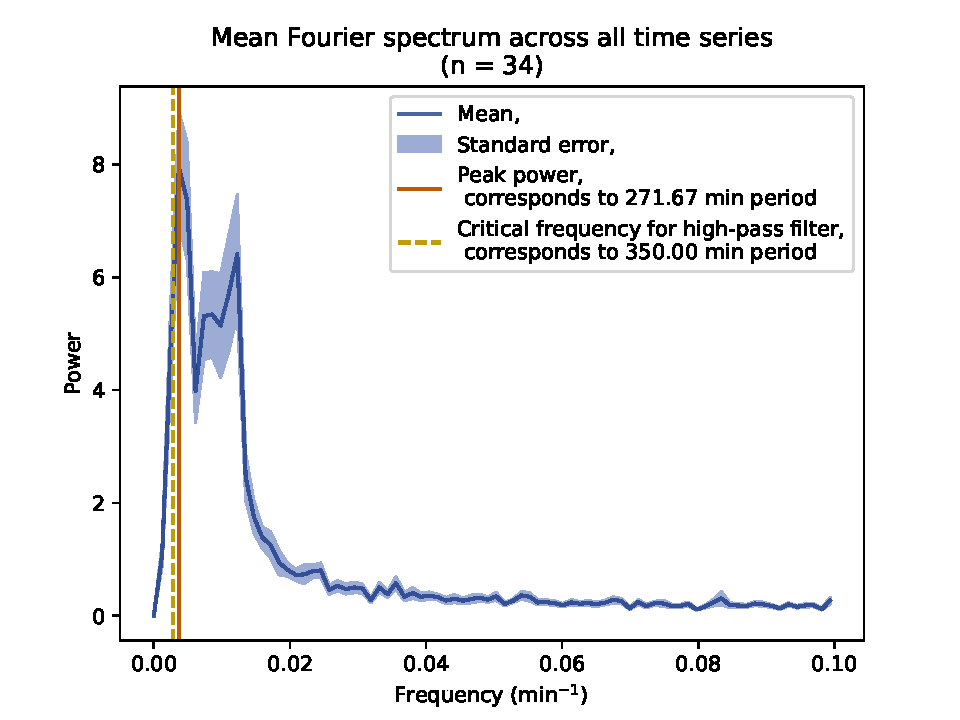
\includegraphics[width=\textwidth]{cenpkkoetter_20212_13.pdf}
   \caption{
   }
   \label{fig:biology-cenpk-sync-fourier}
  \end{subfigure}%
  \begin{subfigure}[htpb]{0.45\textwidth}
   \centering
   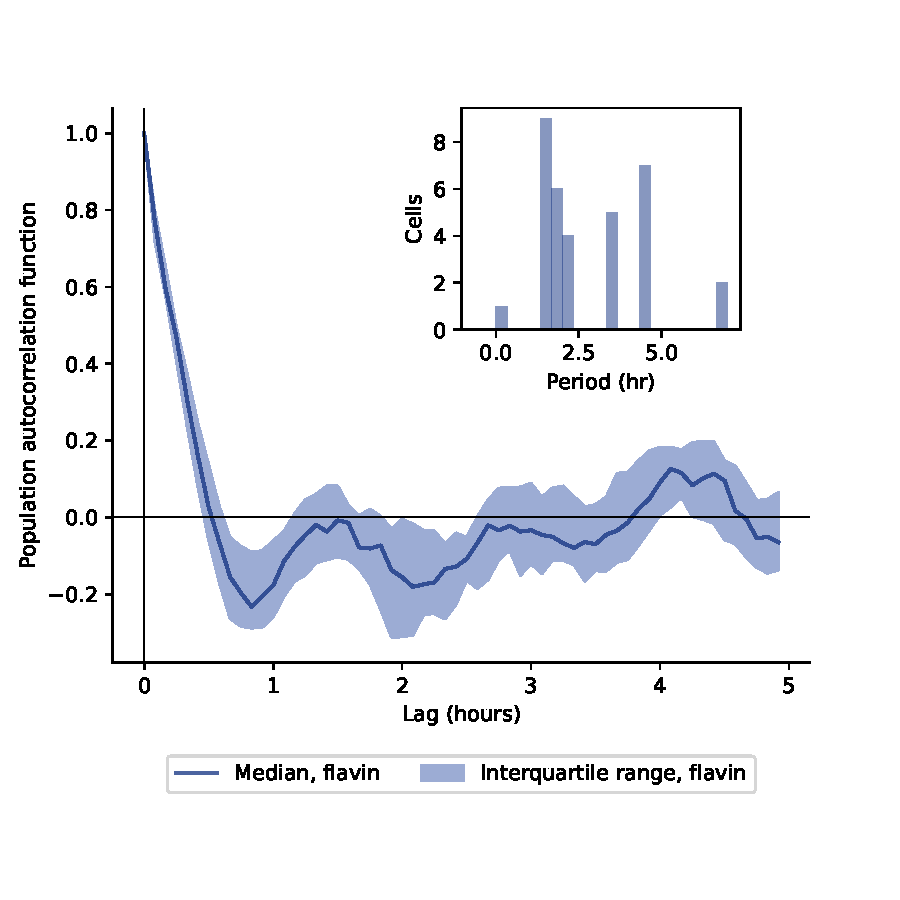
\includegraphics[width=\textwidth]{cenpkkoetter_20212_12.pdf}
   \caption{
   }
   \label{fig:biology-cenpk-sync-acf}
  \end{subfigure}

  % The heatmap looks bad because there were few cells, so omitted.
  % \begin{subfigure}[htpb]{0.45\textwidth}
  %  \centering
  %  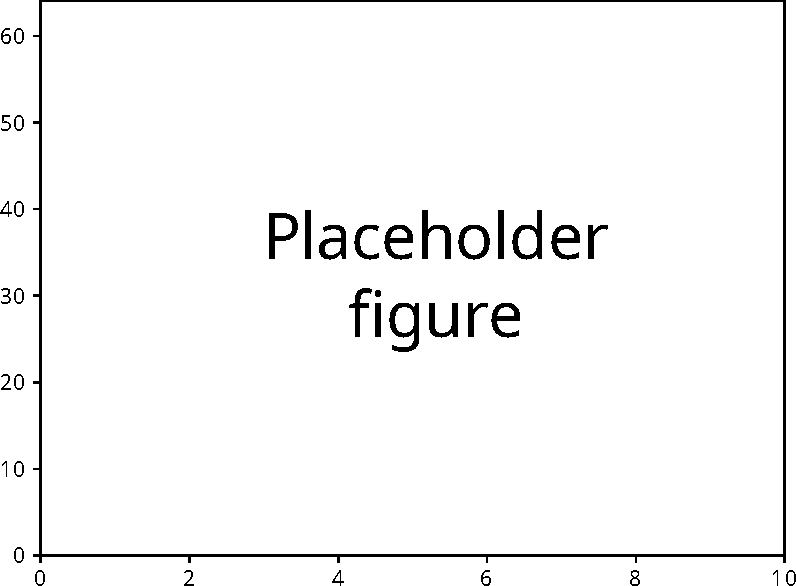
\includegraphics[width=\textwidth]{placeholder03.pdf}
  %  \caption{
  %  }
  %  \label{fig:biology-cenpk-sync-heatmap}
  % \end{subfigure}%
  \begin{subfigure}[htpb]{0.45\textwidth}
   \centering
   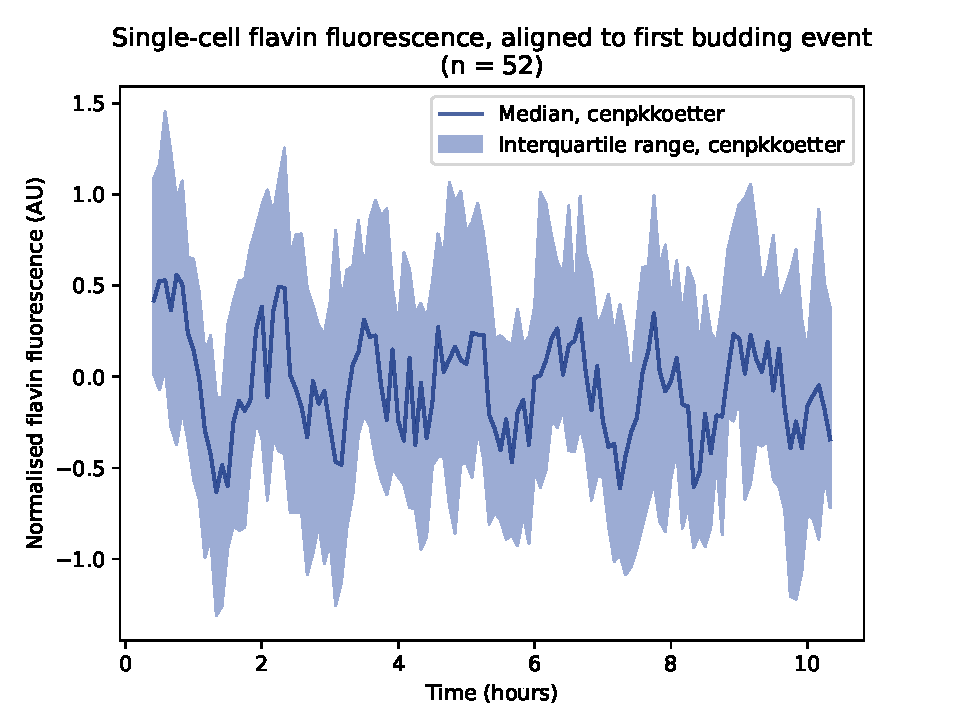
\includegraphics[width=\textwidth]{cenpkkoetter_20212_6.pdf}
   \caption{
   }
   \label{fig:biology-cenpk-sync-median}
  \end{subfigure}

  \caption[
    Mean Fourier spectrum of flavin fluorescence across cells.
    Median autocorrelation function of flavin fluorescence time series, along with the periods across cells.
    Median flavin fluorescence signal across cells, aligned to first budding event.
    Data are from CEN.PK113-7D cells in \SI{10}{\gram~\litre^{-1}} glucose.
  ]{
    \textbf{(\ref{fig:biology-cenpk-sync-fourier})} Mean Fourier spectrum of flavin fluorescence across cells.
    \textbf{(\ref{fig:biology-cenpk-sync-acf})} Median autocorrelation function of flavin fluorescence time series, along with \textit{\textbf{(inset)}} the periods across cells as determined by the frequency with the greatest power in each signal's Fourier spectrum.
    % \textbf{(\ref{fig:biology-cenpk-sync-heatmap})}
    % heatmap showing the flavin fluorescence (pixels on a red-blue scale) and budding events (black pixels) of each cell,
    % signals are aligned by the first budding event; and
    \textbf{(\ref{fig:biology-cenpk-sync-median})}
    Median flavin fluorescence signal across cells, aligned to first budding event.
    Data are from CEN.PK113-7D cells in \SI{10}{\gram~\litre^{-1}} glucose.
  }
  \label{fig:biology-cenpk-sync}
\end{figure}


\section{Metabolic cycles in different carbon sources}
\label{sec:biology-carbon}

To show that the metabolic cycle responds to nutrient conditions and, accordingly, adjusts the cell's metabolism and cell division cycle, I cultured cells in pyruvate and in a growth-limiting glucose concentration.
These experiments are important as they confirm conclusions about varying nutrient conditions made by \textcite{papagiannakisAutonomousMetabolicOscillations2017},
but using flavin autofluorescence.
Specifically, pyruvate provided an example of a non-fermentable carbon source to test whether the switch from fermentative to respiratory metabolism affected the metabolic cycle.
Additionally, a growth-limiting glucose concentration emulated low-glucose concentrations in a chemostat and was thus used to test whether long YMCs observed in such conditions can be replicated in a microfluidics platform.

Fig.\ \ref{fig:biology-pyruvate} shows that FY4 HTB2::mCherry cells had longer metabolic cycles and cell division cycles (approximately \SI{4}{\hour}) when grown in minimal media supplemented with \SI{20}{\gram~\litre^{-1}} pyruvate, compared to growth in high glucose.
%In addition, there were more cases in which the flavin signal peaks without a budding event. %(supplementary figure ...).
Furthermore, the synchrony between the metabolic cycle and cell division cycle remained, but with a longer lag (\SI{60}{\minute}) of the mCherry signal peak with respect to the flavin signal peak (Fig.\ \ref{fig:biology-pyruvate-xcf}).
Fig.\ \ref{fig:biology-pyruvate-single} shows that the longer cell division cycles were because of longer G\textsubscript{1} phases but unchanged S/M phases, as evidenced by the longer flat regions of the mCherry signal.
%However, the flavin cycles were not regular over long periods of time, as evidenced by a lack of repeated oscillations in the cross-correlation function.

\begin{figure}[p]
  \centering
  \begin{subfigure}[htpb]{1.0\textwidth}
   \centering
   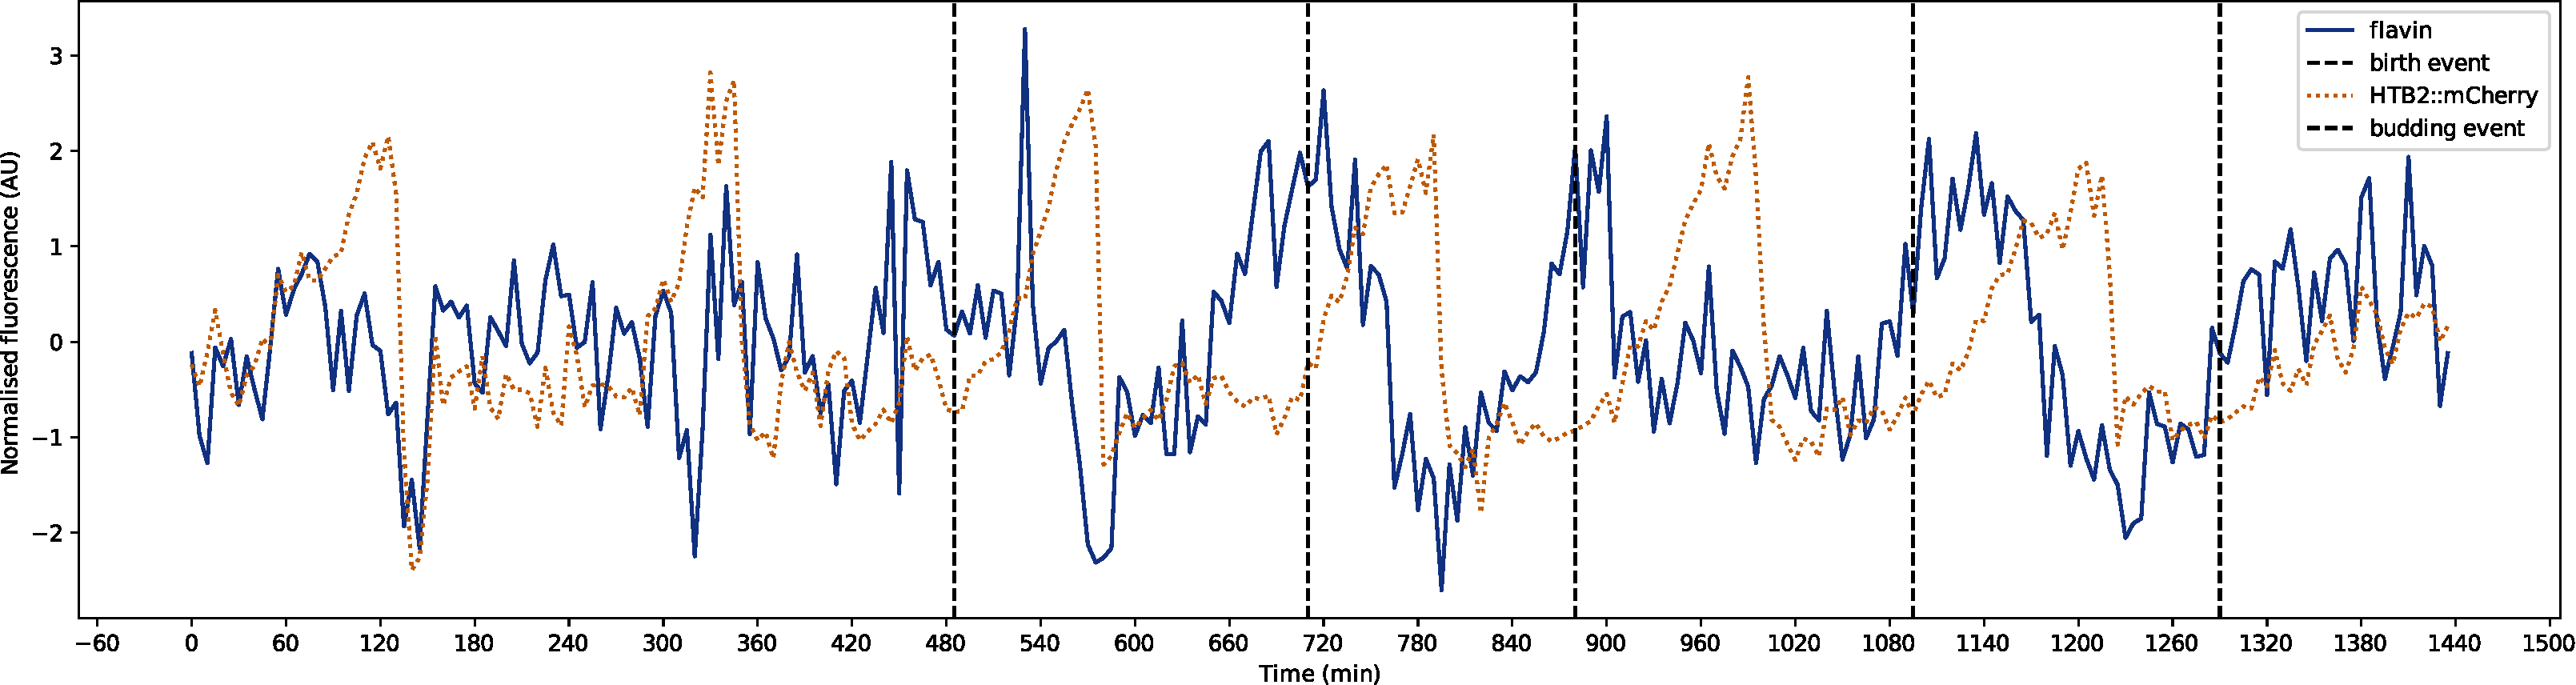
\includegraphics[width=\textwidth]{pyruvate_single_birth_plot_edit.pdf}
   \caption{
     % Oscillations of flavin fluorescence lengthen when cells are cultivated in \SI{20}{\gram~\litre^{-1}} pyruvate while the duration of S/M phase stays constant.
     %Figure shows sample flavin fluorescence levels (purple) and histone 2B localisation (pink) in single cells.
     %Vertical lines (black) indicate budding.
   }
   \label{fig:biology-pyruvate-single}

  \end{subfigure}
  \begin{subfigure}[t]{0.45\textwidth}
   \centering
   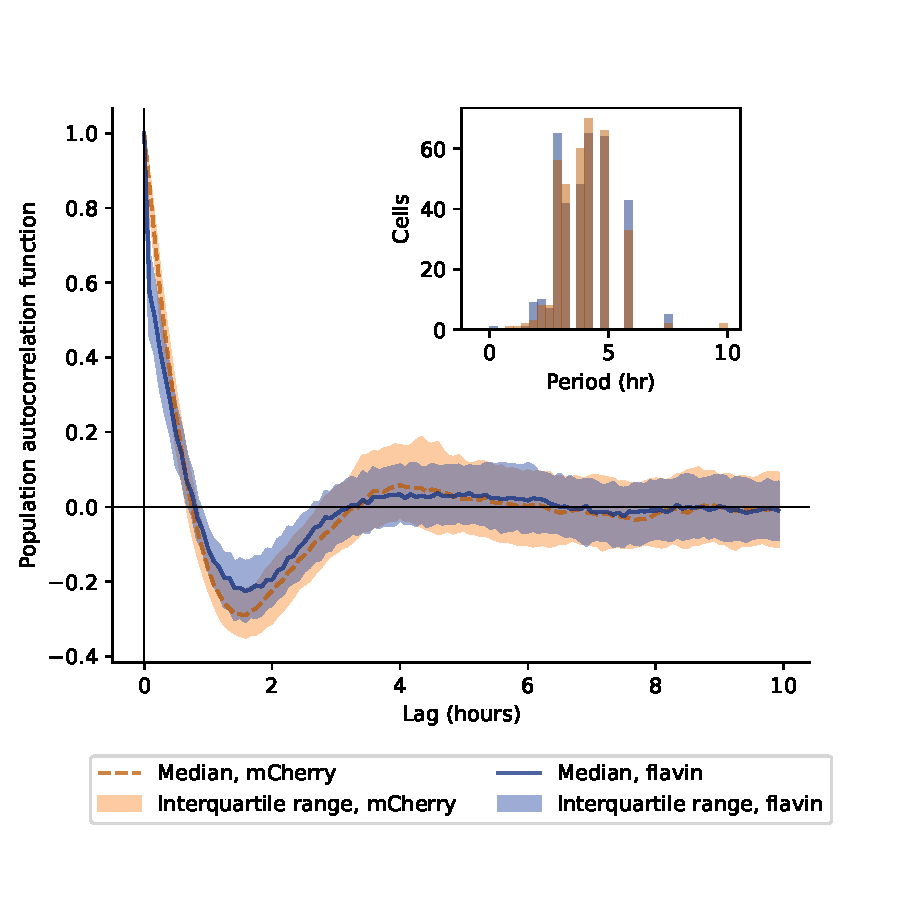
\includegraphics[width=\textwidth]{htb2mCherry_31594_12.pdf}
   \caption{
     % Autocorrelation functions and periods determined by Fourier spectrum of flavin fluorescence and histone 2B levels.
     % This figure indicates that the cells' metabolic cycles and cell division cycles are both consistently approximately 4 hours long.
   }
   \label{fig:biology-pyruvate-acf}
  \end{subfigure}%
  \begin{subfigure}[t]{0.45\textwidth}
   \centering
   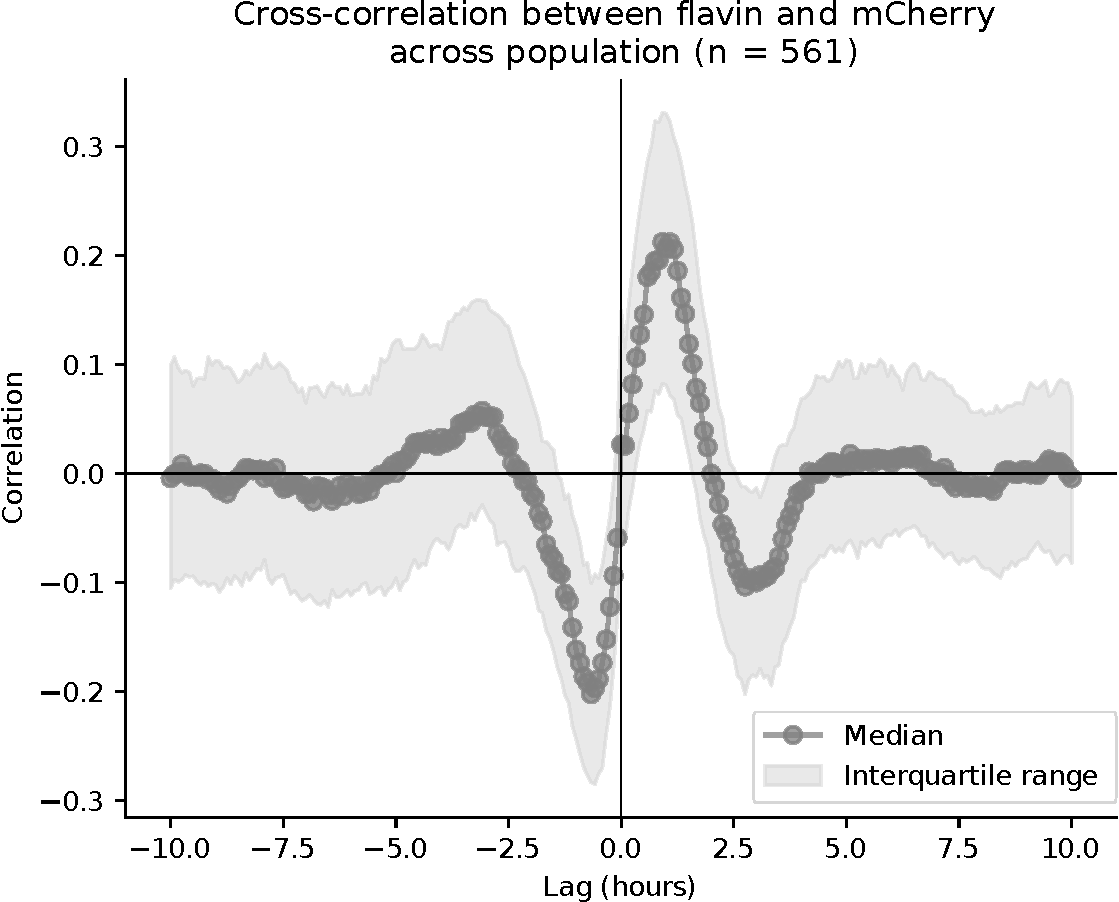
\includegraphics[width=\textwidth]{pyruvate_xcf_edit.pdf}
   \caption{
    %Cross-correlation between flavin and histone 2B signals, indicating that histone levels peak 1 hour after flavin fluorescence peaks.
   }
   \label{fig:biology-pyruvate-xcf}
  \end{subfigure}

  \caption[
    Flavin fluorescence and histone 2B levels in a single, representative FY4 HTB2::mCherry cell grown in \SI{20}{\gram~\litre^{-1}} pyruvate.
    Median autocorrelation functions of flavin fluorescence and histone 2B levels time series, along with the periods of each oscillator across cells.
    Median cross-correlation function between flavin and histone 2B signals.
    Data are from FY4 HTB2::mCherry cells in \SI{20}{\gram~\litre^{-1}} pyruvate.
  ]{
    \textbf{(\ref{fig:biology-pyruvate-single})}
    Flavin fluorescence (blue, solid lines) and histone 2B (orange, dotted lines) levels in a single, representative FY4 HTB2::mCherry cell grown in \SI{20}{\gram~\litre^{-1}} pyruvate.
    Vertical lines (black, dashed) indicate budding events.
    \textbf{(\ref{fig:biology-pyruvate-acf})}
    Median autocorrelation functions of flavin fluorescence (blue) and histone 2B levels (orange) time series, along with \textit{\textbf{(inset)}} the periods of each oscillator across cells as determined by the frequency with the greatest power in each signal's Fourier spectrum.
    \textbf{(\ref{fig:biology-pyruvate-xcf})}
    Median cross-correlation function between flavin and histone 2B signals.
    Data are from FY4 HTB2::mCherry cells in \SI{20}{\gram~\litre^{-1}} pyruvate.
  }
  \label{fig:biology-pyruvate}
\end{figure}

% COULD DO:
% (Add statistical tests to reject the null hypothesis that the mean duration of metabolic cycles in pyruvate is equal to the mean duration of metabolic cycles in high glucose.  This would depend on having a good number of the duration, and it looks like the inset is the best candidate for this.)

\pagebreak

Fig.\ \ref{fig:biology-lowglc} shows that FY4 HTB2::mCherry cells had longer metabolic cycles when grown in minimal media supplemented with \SI{0.010}{\gram~\litre^{-1}} glucose.

\begin{figure}[b!]
  \centering
  \begin{subfigure}[htpb]{1.0\textwidth}
   \centering
   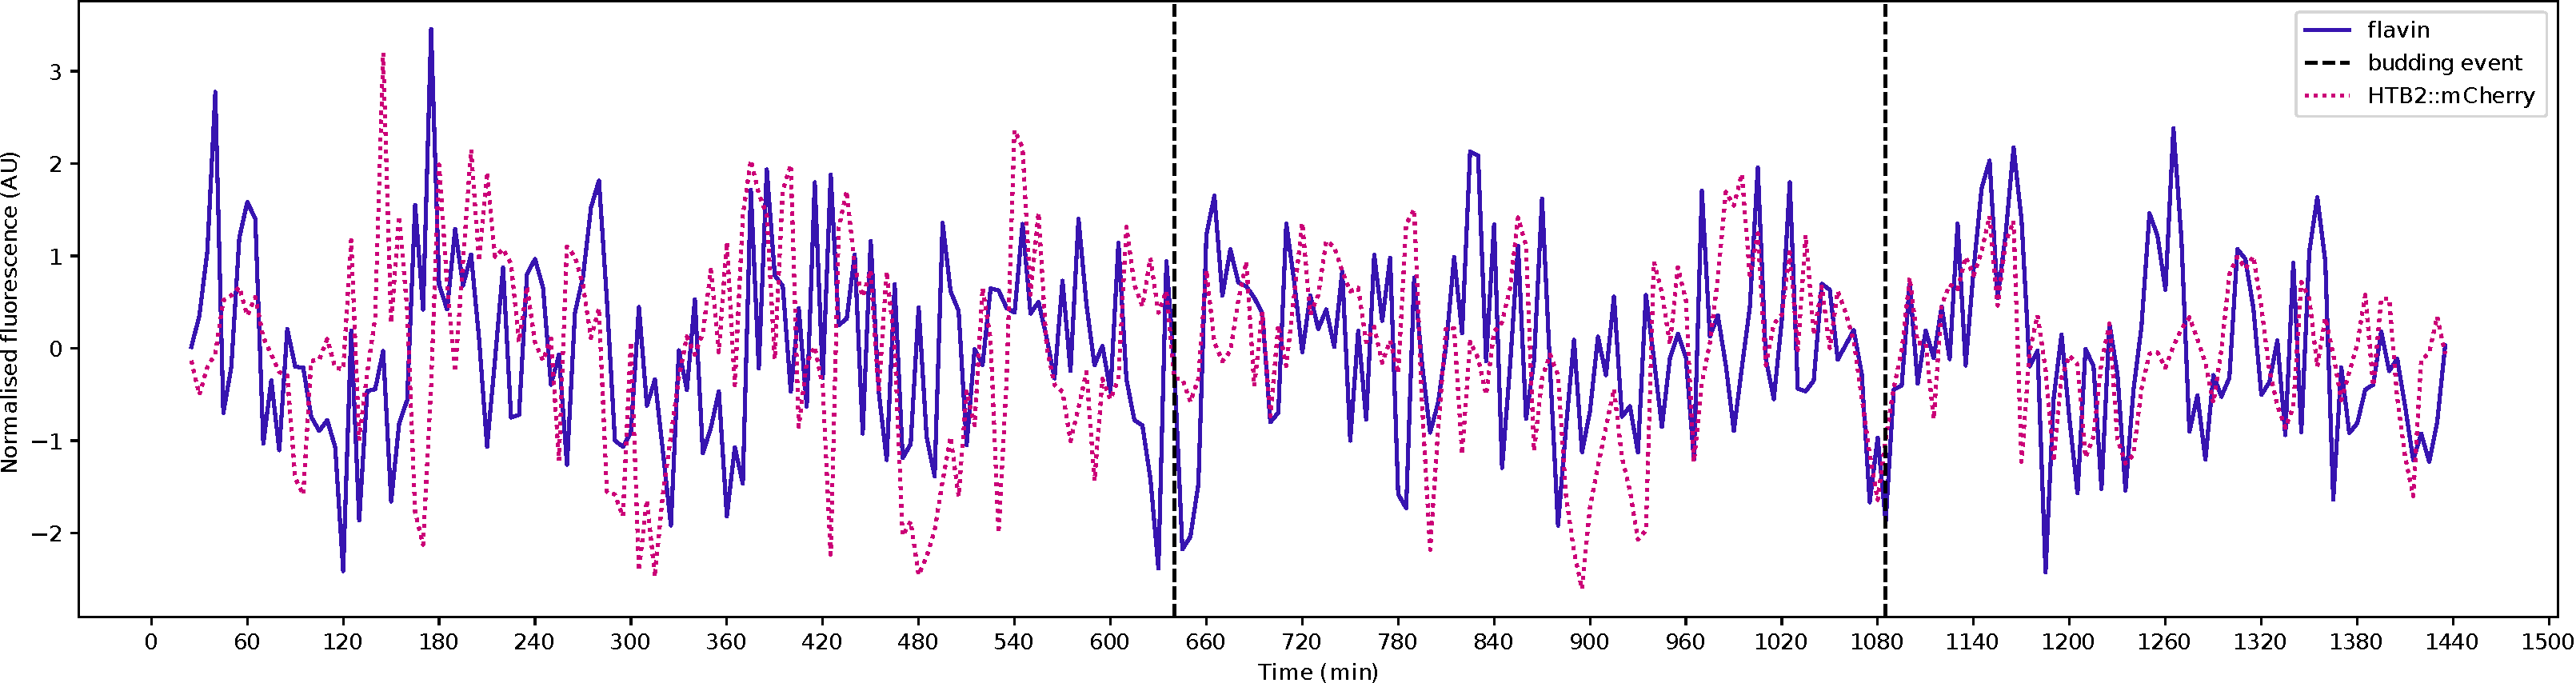
\includegraphics[width=\textwidth]{limiting_single_birth_plot_edit.pdf}
   \caption{
   }
   \label{fig:biology-lowglc-single}
  \end{subfigure}

  \begin{subfigure}[htpb]{0.7\textwidth}
   \centering
   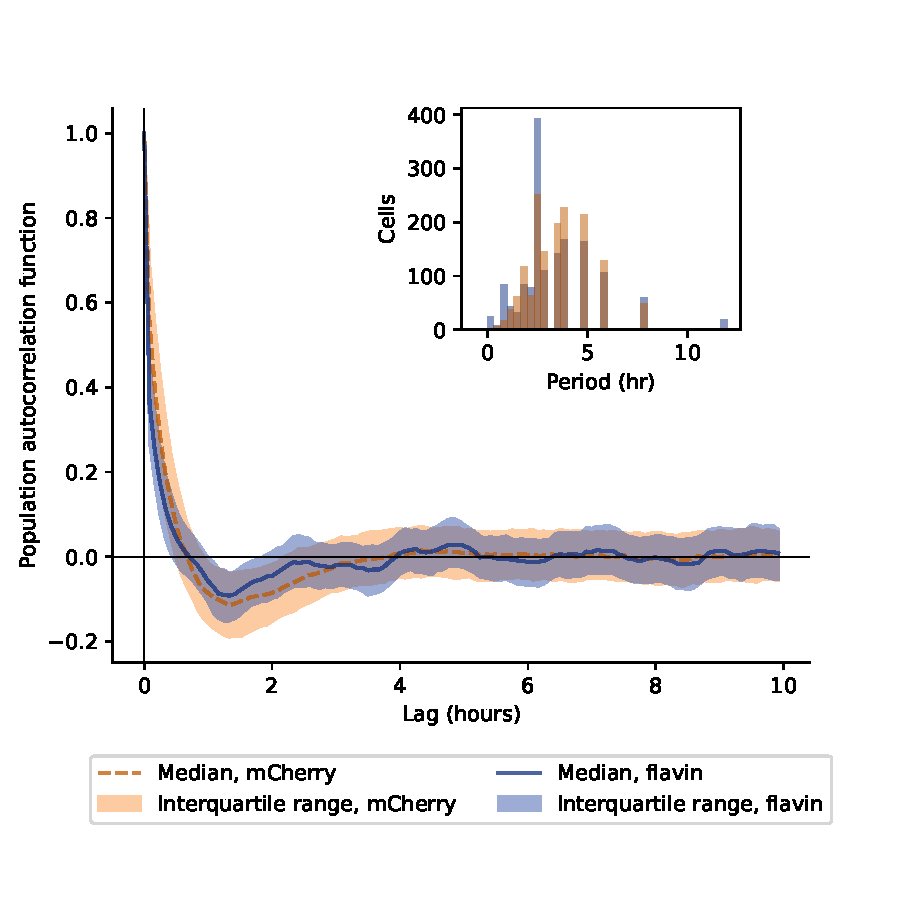
\includegraphics[width=\textwidth]{htb2mCherry_31492_12.pdf}
   \caption{
   }
   \label{fig:biology-lowglc-acf}
  \end{subfigure}
  \caption[
    Flavin fluorescence and histone 2B levels in a single, representative FY4 HTB2::mCherry cell grown in \SI{0.010}{\gram~\litre^{-1}} glucose.
    Median autocorrelation functions of flavin fluorescence and histone 2B levels time series, along with  the periods of each oscillator across cells.
    Data are from FY4 HTB2::mCherry cells in \SI{0.010}{\gram~\litre^{-1}} glucose.
  ]{
    \textbf{(\ref{fig:biology-lowglc-single})}
    Flavin fluorescence (blue, solid lines) and histone 2B (orange, dotted lines) levels in a single, representative FY4 HTB2::mCherry cell grown in \SI{0.010}{\gram~\litre^{-1}} glucose.
    Vertical lines (black, dashed) indicate budding events.
    \textbf{(\ref{fig:biology-lowglc-acf})}
    Median autocorrelation functions of flavin fluorescence (blue) and histone 2B levels (orange) time series, along with \textit{\textbf{(inset)}} the periods of each oscillator across cells as determined by the frequency with the greatest power in each signal's Fourier spectrum.
    Data are from FY4 HTB2::mCherry cells in \SI{0.010}{\gram~\litre^{-1}} glucose.
  }
  \label{fig:biology-lowglc}
\end{figure}

\pagebreak

Additionally, Fig.\ \ref{fig:biology-lowglc-gr-budprob} shows that the growth rate and the rate of bud formation of cells on limiting glucose was lower than on high glucose (\SI{20}{\gram~\litre^{-1}}).

\begin{figure}[htbp!]
  \centering
  \begin{subfigure}[htpb]{0.45\textwidth}
   \centering
   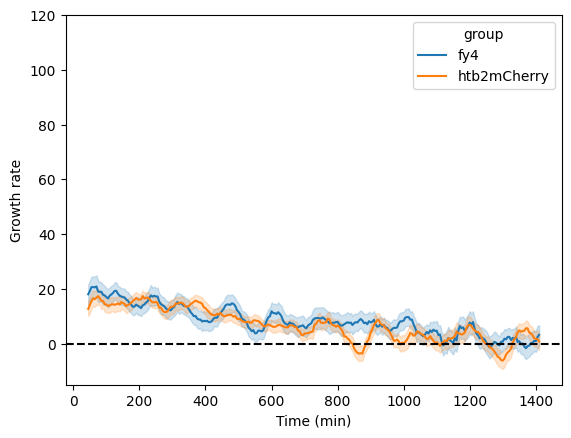
\includegraphics[width=\textwidth]{allstrains_31492_gr}
   \caption{
   }
   \label{fig:biology-lowglc-gr}
  \end{subfigure}%
  \begin{subfigure}[htpb]{0.45\textwidth}
   \centering
   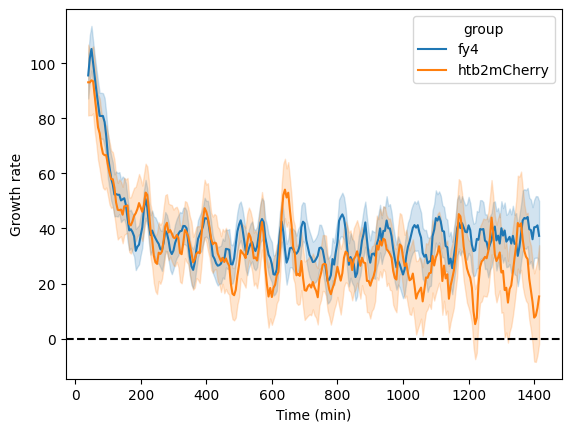
\includegraphics[width=\textwidth]{allstrains_26643_gr}
   \caption{
   }
   \label{fig:biology-highglc-gr}
  \end{subfigure}

  \begin{subfigure}[htpb]{0.45\textwidth}
   \centering
   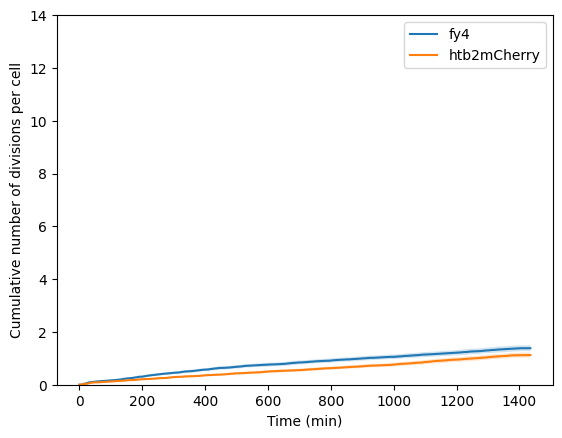
\includegraphics[width=\textwidth]{allstrains_31492_cumul}
   \caption{
   }
   \label{fig:biology-lowglc-cumul}
  \end{subfigure}%
  \begin{subfigure}[htpb]{0.45\textwidth}
   \centering
   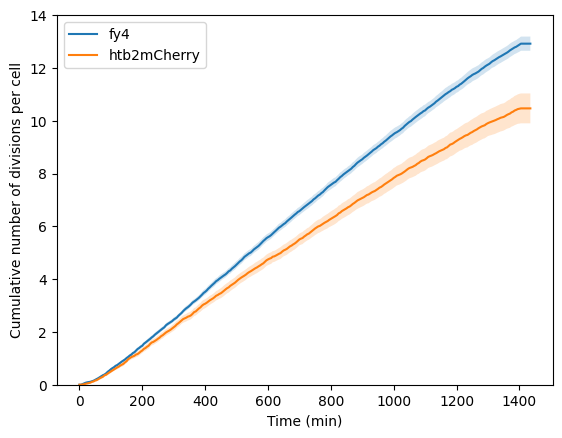
\includegraphics[width=\textwidth]{allstrains_26643_cumul}
   \caption{
   }
   \label{fig:biology-highglc-cumul}
  \end{subfigure}

  \caption[
    Mean growth rate, derived from changes in the sum of estimated parent cell and bud volumes
    of FY4 and HTB2::mCherry strains over time during the glucose-starvation experiment, for
    the glucose-limiting condition and
    the high glucose condition.
    Similarly, the mean cumulative number of budding events per cell.
  ]{
    Mean growth rate, derived from changes in the sum of estimated parent cell and bud volumes (shading: 95\% confidence intervals) of FY4 (blue) and HTB2::mCherry (orange) strains over time, for \textbf{(\ref{fig:biology-lowglc-gr})} the glucose-limiting condition (\SI{0.010}{\gram~\litre^{-1}}) and \textbf{(\ref{fig:biology-highglc-gr})} the high glucose condition (\SI{20}{\gram~\litre^{-1}}).
    Similarly, the mean cumulative number of budding events per cell (shading: confidence intervals from bootstrapping, $n=30$), of the same strains for \textbf{(\ref{fig:biology-lowglc-cumul})} the glucose-limiting condition and \textbf{(\ref{fig:biology-highglc-cumul})} the high glucose condition.
  }
  \label{fig:biology-lowglc-gr-budprob}
\end{figure}

Furthermore, Fig.\ \ref{fig:biology-compare-snr} shows that the amplitude of the flavin oscillations in this glucose-limiting condition was low relative to other conditions, as evidenced by the lower signal-to-noise ratios (two-sided Kolmogorov-Smirnov test: low-glucose vs pyruvate $p = \num{1.6e-82}$, low-glucose vs high-glucose $p = \num{1.9d-171}$).

\begin{figure}[htbp!]
  \centering
  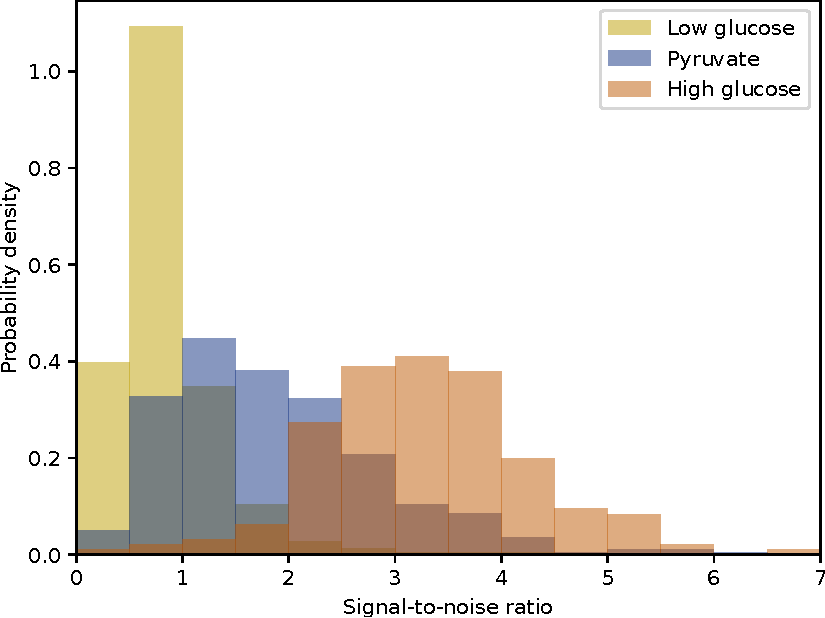
\includegraphics[width=0.6\textwidth]{csource_snrs_edit}

  \caption{
    Distributions of signal-to-noise ratios of flavin signals from cells in
    (yellow) \SI{0.010}{\gram~\litre^{-1}} glucose,
    (blue) \SI{20}{\gram~\litre^{-1}} pyruvate, and
    (orange) \SI{20}{\gram~\litre^{-1}} glucose.
    Vertical axis shows probability density, computed by dividing the number of cells in each bin by the total number of cells and then by the bin width.
  }
  \label{fig:biology-compare-snr}
\end{figure}

Finally, Fig.\ \ref{fig:biology-lowglc-acf} shows that measurements of the metabolic cycle and the cell division cycle lost synchrony in limiting glucose.
This was evidenced by a \SI{2.5}{\hour} average metabolic cycle, though not robust, but an absence of consistent oscillations in mCherry intensity.
This decoupling can be explained by a lack of cell division cycle events.

% In contrast to 20 g/L glucose in which metabolic cycles were asynchronous, in these conditions there is some degree of metabolic cycle synchrony between cells. \textbf{(add figures)}

% TODO: How are these linked to Papagiannakis et al.?  Am I getting the same conclusions?  Also -- space to discuss the 10-hour oscillations in chemostats in slow dilution rates.


%\section[Potassium-deficient media]{Do single-cell flavin traces recapitulate dissolved-oxygen YMCs in chemostats? -- potassium-deficient media}
\section{Metabolic cycles persist in potassium-deficient media}
\label{sec:biology-potassium_deficient}

To address whether single-cell flavin traces from microfluidic experiments recapitulate dissolved-oxygen yeast metabolic cycles in chemostats, I replicated conditions of chemostat-based studies in which nutrient or genetic perturbations severely affected the metabolic cycle.
These nutrient conditions included potassium deficiency and deletion strains included \textit{zwf1$\Delta$} and \textit{tsa1$\Delta$ tsa2$\Delta$}.
Replicating conditions of chemostat-based studies is important in showing that the single-cell metabolic cycle and the chemostat metabolic cycle are the same cycle, or to prove otherwise.
Chemostat experiments obscure the behaviour of individual cells, and single-cell microfluidics experiments can provide a bottom-up explanation of high-level observations of the metabolic cycle in the chemostat. Such single-cell experiments could address, for example, whether the cellular behaviour of the yeast metabolic cycle explains the changes in dissolved-oxygen oscillations.

To test whether potassium deficiency eliminates metabolic cycles, I treated cells with potassium-deficient minimal medium, replacing monopotassium phosphate (\ce{KH2PO4}) in the minimal medium with an equivalent molarity of monosodium phosphate (\ce{NaH2PO4}), as described in Table~\ref{tab:methods-media-delft}, with both media supplemented with \SI{20}{\gram~\litre^{-1}} glucose as a carbon source.
\textcite{oneillEukaryoticCellBiology2020} suggested that, in chemostat cultures, as potassium in the nutrient medium is gradually replaced with sodium, the period and amplitude of dissolved-oxygen oscillations decrease until the oscillations disappear (Fig.\ \ref{fig:biology-kdeficient-oneill}).

\begin{figure}[hb!]
  \centering
  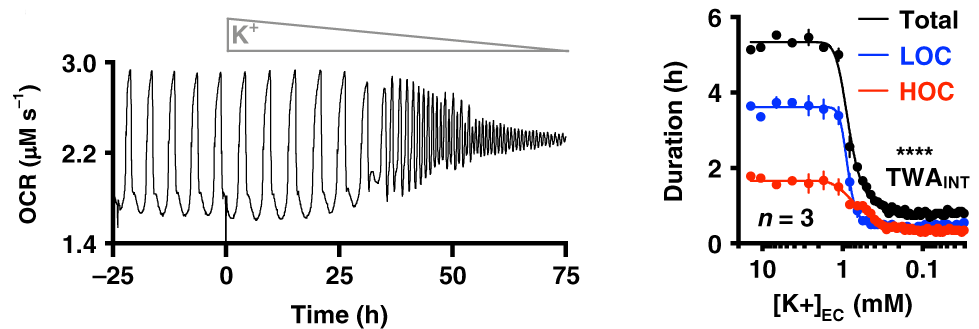
\includegraphics[width=0.7\textwidth]{oneillEukaryoticCellBiology2020_4_adapted.png}
  \caption{
    Decreasing extracellular potassium (\ce{K+}) concentration shortens, then under \SI{1}{\milli\molar}, destroys metabolic oscillations in the chemostat.
    Adapted from \textcite{oneillEukaryoticCellBiology2020}.
  }
  \label{fig:biology-kdeficient-oneill}
\end{figure}

Fig.\ \ref{fig:biology-kdeficient-single} shows that FY4 HTB2::mCherry cells retained synchronised metabolic cycles and cell division cycles when cells were abruptly switched from potassium-containing to potassium-deficient minimal medium.
Such cycles were longer and were generated less reliably as in the normal growth medium (Fig.\ \ref{fig:biology-kdeficient-acf}).

\begin{figure}[p]
  \centering
  \begin{subfigure}[htpb]{1.0\textwidth}
   \centering
   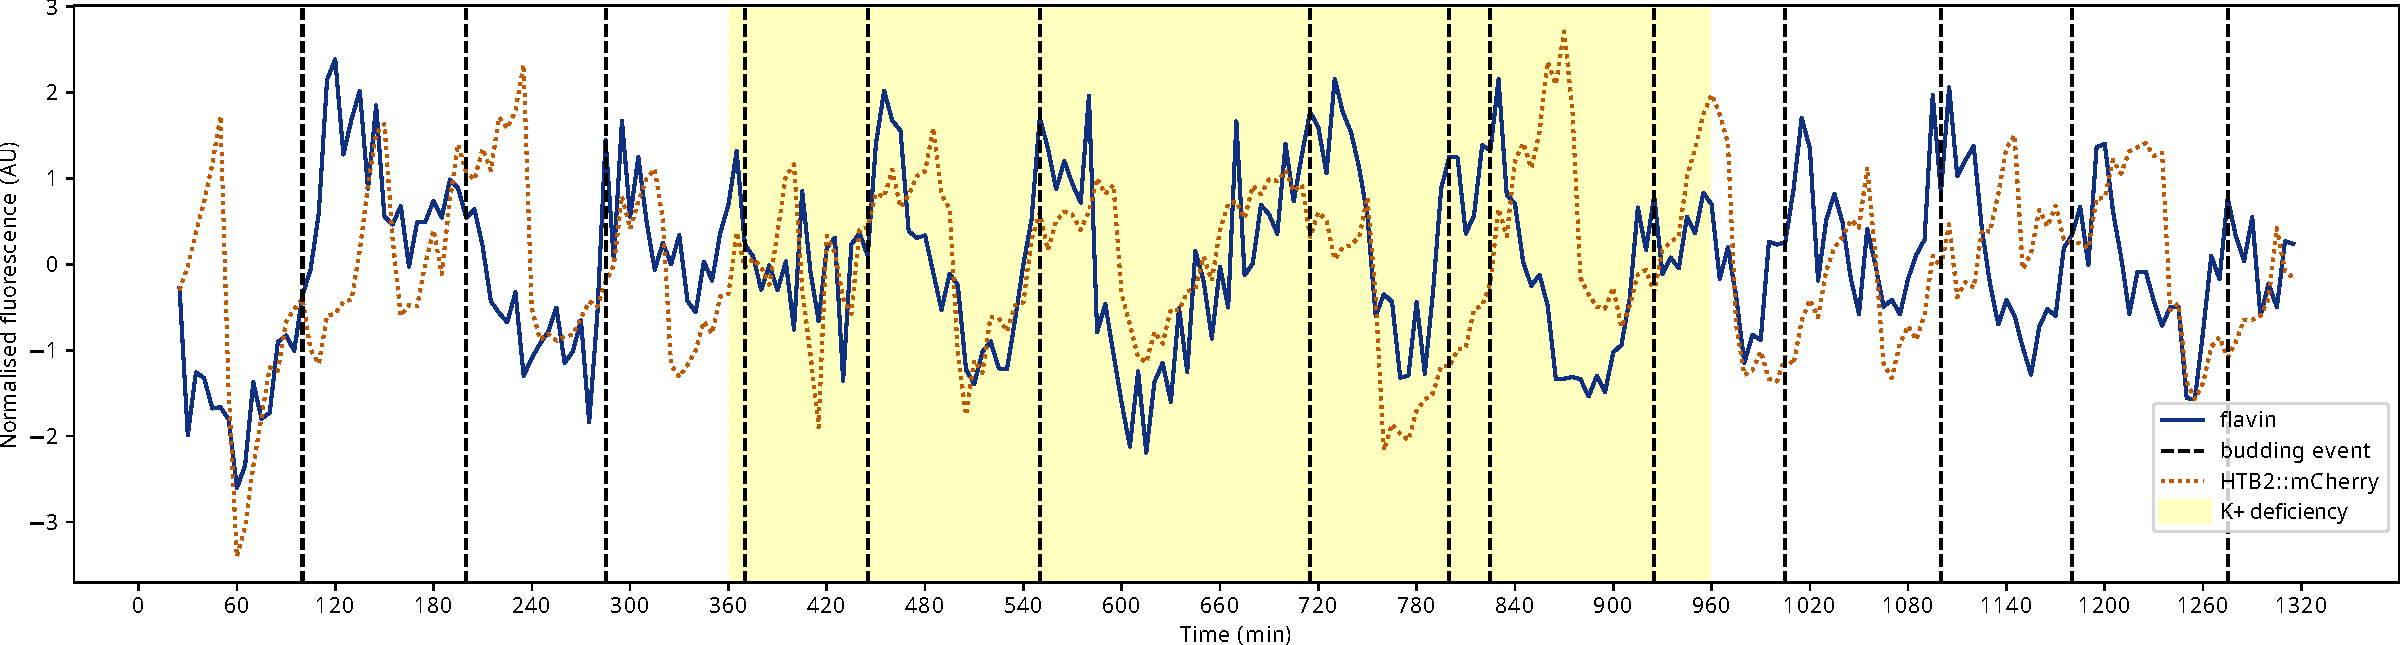
\includegraphics[width=\textwidth]{htb2mCherry_613_plots_single_htb2mCherry012_90_2_adapted.pdf}
   \caption{
   }
   \label{fig:biology-kdeficient-single}
  \end{subfigure}

  \begin{subfigure}[htpb]{0.7\textwidth}
   \centering
   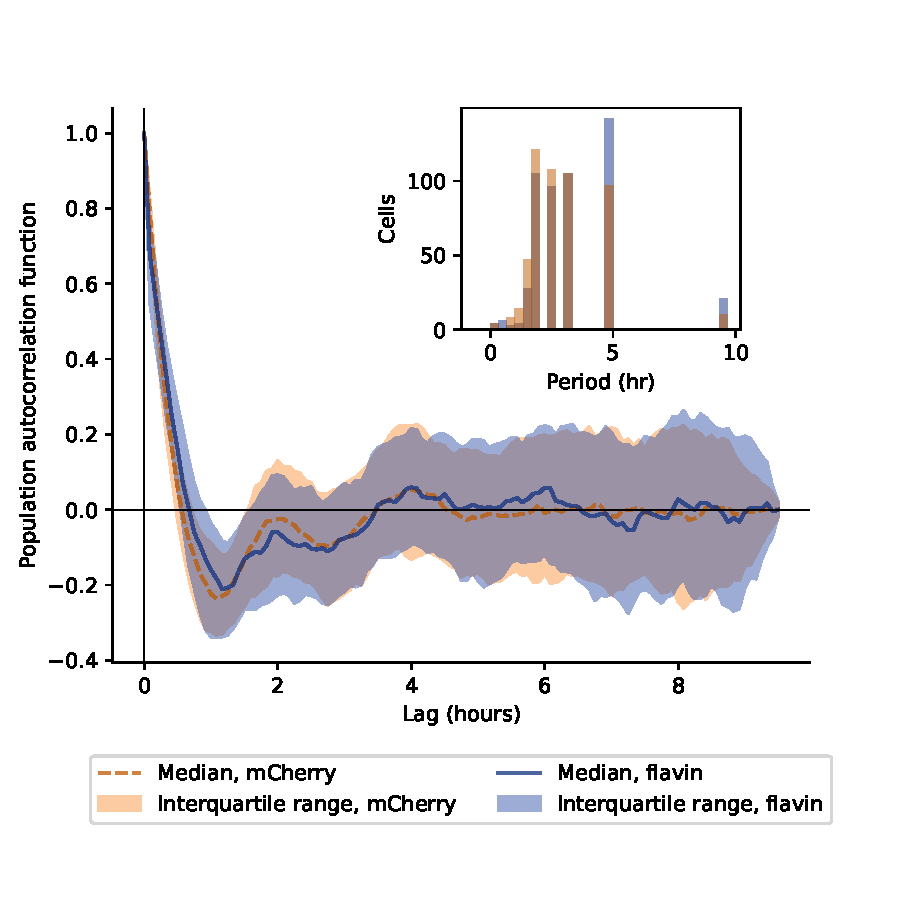
\includegraphics[width=\textwidth]{htb2mCherry_613_12.pdf}
   \caption{
   }
   \label{fig:biology-kdeficient-acf}
  \end{subfigure}

  \caption[
    Flavin fluorescence and histone 2B levels in a single, representative FY4 HTB2::mCherry cell.
    Median autocorrelation functions of flavin fluorescence and histone 2B levels time series, along with  the periods of each oscillator across cells.
    Data are from FY4 and HTB2::mCherry cells; autocorrelation functions only used time points from the potassium-deficient condition.
  ]{
    \textbf{(\ref{fig:biology-kdeficient-single})}
    Flavin fluorescence (blue, solid lines) and histone 2B (orange, dotted lines) levels in a single, representative FY4 HTB2::mCherry cell.
    Vertical lines (black, dashed) indicate budding events.
    Shading (yellow) indicates the potassium-deficient period.
    \textbf{(\ref{fig:biology-kdeficient-acf})}
    Median autocorrelation functions of flavin fluorescence (blue) and histone 2B levels (orange) time series, along with \textit{\textbf{(inset)}} the periods of each oscillator across cells as determined by the frequency with the greatest power in each signal's Fourier spectrum.
    Data are from FY4 and HTB2::mCherry cells; autocorrelation functions only used time points from the potassium-deficient condition (\SIrange{6}{16}{\hour}).
  }
  \label{fig:biology-kdeficient}
\end{figure}

In addition, the distribution of signal-to-noise ratios of time series before potassium-deficiency and during potassium-deficiency were identical (Fig.\ \ref{fig:biology-kdeficient-snr}; two-sided Kolmogorov-Smirnov test, $p = \num{0.10}$), indicating an unchanged amplitude of flavin signal; however, the same was not true when comparing time series during potassium-deficiency and after potassium-deficiency (two-sided Kolmogorov-Smirnov test, $p = \num{4.09e-7}$).
%Furthermore, although the changes in the mean signal-to-noise ratio as the medium changed were significant (Fig.\ \ref{fig:biology-kdeficient-snr}; $\bar{x}_{\mathrm{before}} = 2.22$, $\bar{x}_{\mathrm{deficient}} = 2.44$, $\bar{x}_{\mathrm{after}} = 1.79$; Welch's $t$-test: deficient vs before $p = \num{0.015}$, deficient vs after $p = \num{1.26d-12}$), the differences were more subtle than in the glucose-starvation experiment.

\begin{figure}[hb!]
  \centering
   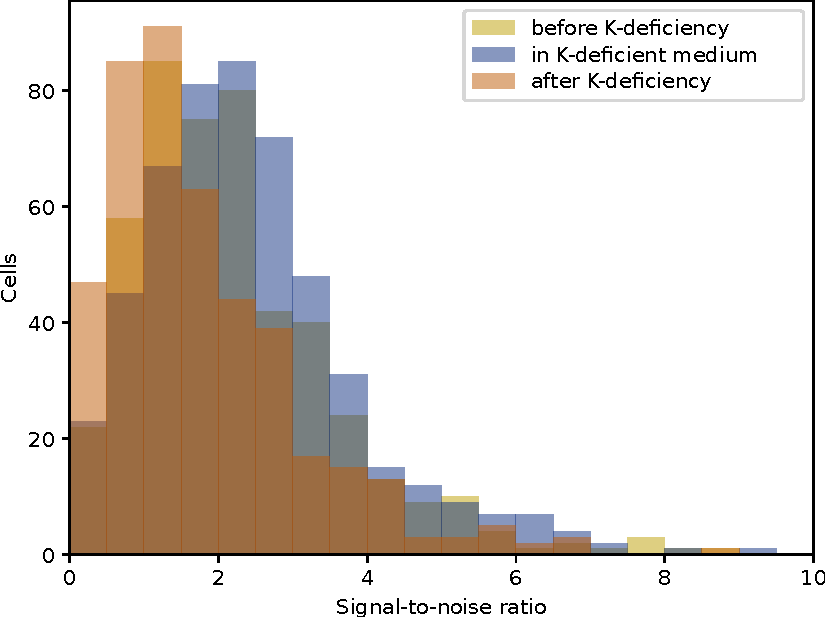
\includegraphics[width=0.6\textwidth]{kdeficient_snr_edit.pdf}
   \caption{
     Distributions of signal-to-noise ratios of flavin signals from cells before, during, and after potassium-deficiency.
   }
  \label{fig:biology-kdeficient-snr}
\end{figure}

In addition, to test whether potassium deficiency affected cell growth and division, Fig.\ \ref{fig:biology-kdeficient-gr} shows that growth rates recovered soon after a sharp decrease upon the abrupt switch to the potassium-deficient medium.
This global response across cells is suggestive of an osmotic response as a result of intracellular potassium leaking out the cell, though the change and recovery of growth rate is slower than the change and recovery of cell volume in response to osmotic stress reported by \textcite{granadosDistributingTasksMultiple2017}.
Fig.\ \ref{fig:biology-kdeficient-cumul} further shows that the rate of budding was unaffected during potassium-deficiency, in contrast to a pause under glucose starvation (Fig.\ \ref{fig:biology-starvation-cumul}).

\begin{figure}[ht!]
  \centering
  \begin{subfigure}[htpb]{0.45\textwidth}
   \centering
   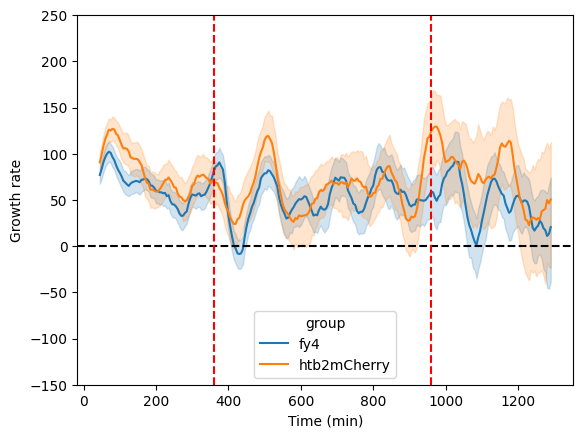
\includegraphics[width=\textwidth]{allstrains_613_gr}
   \caption{
   }
   \label{fig:biology-kdeficient-gr}
  \end{subfigure}%
  \begin{subfigure}[htpb]{0.45\textwidth}
   \centering
   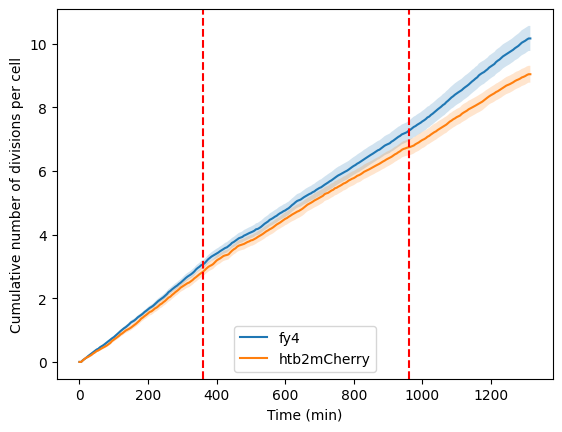
\includegraphics[width=\textwidth]{allstrains_613_cumul}
   \caption{
   }
   \label{fig:biology-kdeficient-cumul}
  \end{subfigure}

  \caption[
    Mean growth rate, derived from changes in the sum of estimated parent cell and bud volumes and
    mean cumulative number of budding events per cell
    of FY4 and HTB2::mCherry strains over time during the potassium-deficient experiment.
  ]{
    \textbf{(\ref{fig:biology-kdeficient-gr})}
    Mean growth rate, derived from changes in the sum of estimated parent cell and bud volumes (shading: 95\% confidence intervals) and
    \textbf{(\ref{fig:biology-kdeficient-cumul})}
    mean cumulative number of budding events per cell (shading: confidence intervals from bootstrapping, $n=30$)
    of FY4 (blue) and HTB2::mCherry (orange) strains over time during the potassium-deficient experiment.
    Vertical lines (red) show changes in the nutrient medium.
  }
  \label{fig:biology-kdeficient-gr-budprob}
\end{figure}

Finally, in contrast to glucose starvation, Fig.\ \ref{fig:biology-kdeficient-histogram} suggests that potassium deficiency did not affect the time each cell spent in each phase of the metabolic and cell division cycles as they progressed through growth.

\begin{figure}[hb!]
  \centering
  \begin{subfigure}[htpb]{0.5\textwidth}
   \centering
   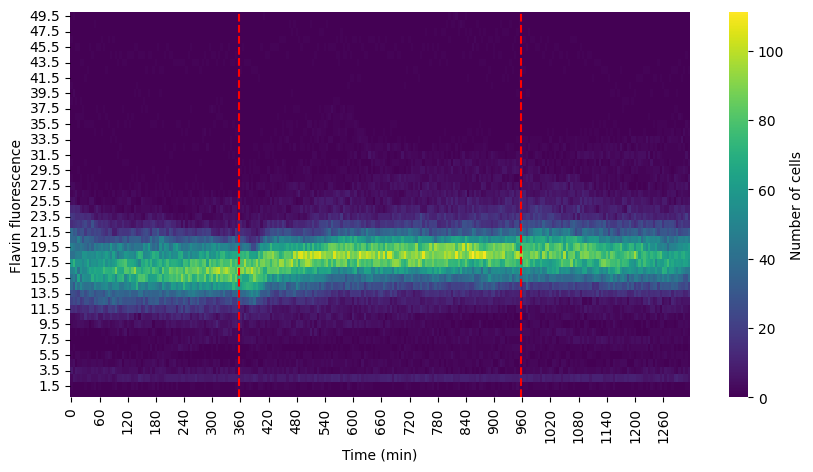
\includegraphics[width=\textwidth]{613_distribs_flavin.png}
   \caption{
   }
   \label{fig:biology-kdeficient-histogram-flavin}
  \end{subfigure}%
  \begin{subfigure}[htpb]{0.5\textwidth}
   \centering
   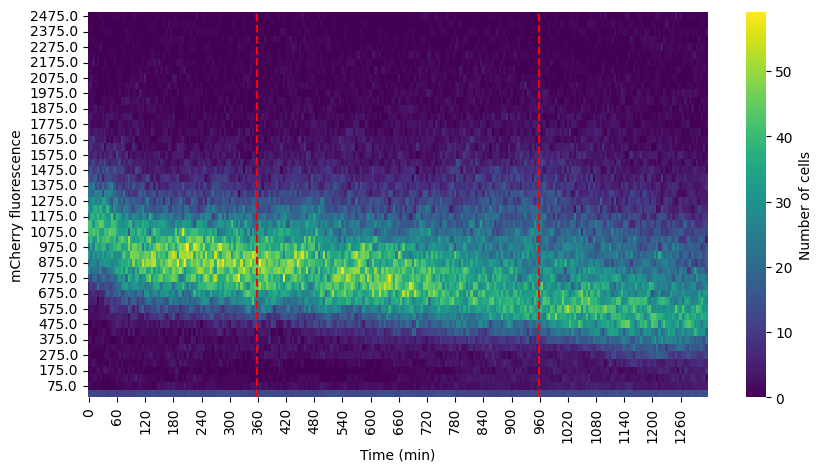
\includegraphics[width=\textwidth]{613_distribs_mCherry.png}
   \caption{
   }
   \label{fig:biology-kdeficient-histogram-mCherry}
  \end{subfigure}

  \caption[
    Distributions of flavin and mCherry fluorescence over time, for the potassium-deficient experiment.
  ]{
    Distributions of \textbf{(\ref{fig:biology-kdeficient-histogram-flavin})} flavin and \textbf{(\ref{fig:biology-kdeficient-histogram-mCherry})} mCherry fluorescence over time, for the potassium-deficient experiment.
    Vertical lines (red, dashed), indicate times of medium changes.
    Raw time series were used to calculate the distributions.
  }
  \label{fig:biology-kdeficient-histogram}
\end{figure}

My results thus show that even though there was an initial response to potassium depletion, cells resumed growth, division, and generation of metabolic cycles soon after.
My observations indicate that the metabolic cycle still occurs with a consistent amplitude, as evidenced by signal-to-noise ratios, in a drastically changed nutrient condition, in contrast to \textcite{oneillEukaryoticCellBiology2020}.
%Thus, my observations warrant a model to reconcile the apparent differences between the chemostat and single-cell investigations.
Furthermore, the significance of the potassium-deficient, sodium-containing nutrient condition is highlighted by the toxicity of sodium ions for budding yeast \parencite{arinoAlkaliMetalCation2010,caseyEffectSaltsCofermentation2013,watcharawipasSodiumAcetateResponses2018}.


%\section[Deletion strains]{Do single-cell flavin traces recapitulate dissolved-oxygen YMCs in chemostats? -- deletion strains}
\section{Metabolic cycles in deletion strains}
\label{sec:biology-deletions}

% \item swe1$\Delta$: gene responsible for CDC processes (another biological rhythm) e.g. DNA repair.  Deletion shown to affect CDC-YMC coupling.
% \item rim11$\Delta$: gene involved in circadian rhythm (another biological rhythm).  Deletion strain shown to have shorter YMCs.

To continue the investigation of whether single-cell flavin-based metabolic cycles recapitulate dissolved-oxygen metabolic cycles, I investigated the \textit{zwf1$\Delta$} and \textit{tsa1$\Delta$ tsa2$\Delta$} deletion strains.
The investigation of deletion strains is important as they can lead to mechanistic explanations of the YMC\@.

To investigate whether the \textit{zwf1$\Delta$} strain shows abolition of the metabolic cycle in single-cell microfluidics, I used a \textit{zwf1$\Delta$} strain with the BY4741 background.
Chemostat-based studies have suggested that in the \textit{zwf1$\Delta$} strain, metabolic cycles are abolished but with little change in growth rate \parencite{tuCyclicChangesMetabolic2007}.
% Move to methods?
Cells were pre-cultured in \SI{20}{\gram~\litre^{-1}} pyruvate over \SI{48}{\hour} and then cultured in \SI{10}{\gram~\litre^{-1}} glucose in the microfluidic device because higher glucose concentrations disfavour growth in this strain.
As the strain had an auxotrophic background, the required nutrient supplements were also added.
%
Fig.\ \ref{fig:biology-zwf1} shows that the \textit{zwf1$\Delta$} cells showed oscillations of approximately \SI{3}{\hour}, but with low robustness and a wide distribution of signal-to-noise ratios, while the reference BY4741 strain showed robust flavin oscillations of approximately \SI{1.5}{\hour}.
These results conflict with the results from the chemostat-based study \parencite{tuCyclicChangesMetabolic2007} that suggested that metabolic cycles are abolished in this strain.

\begin{figure}
  \centering
  \begin{subfigure}[t]{1.0\textwidth}
   \centering
   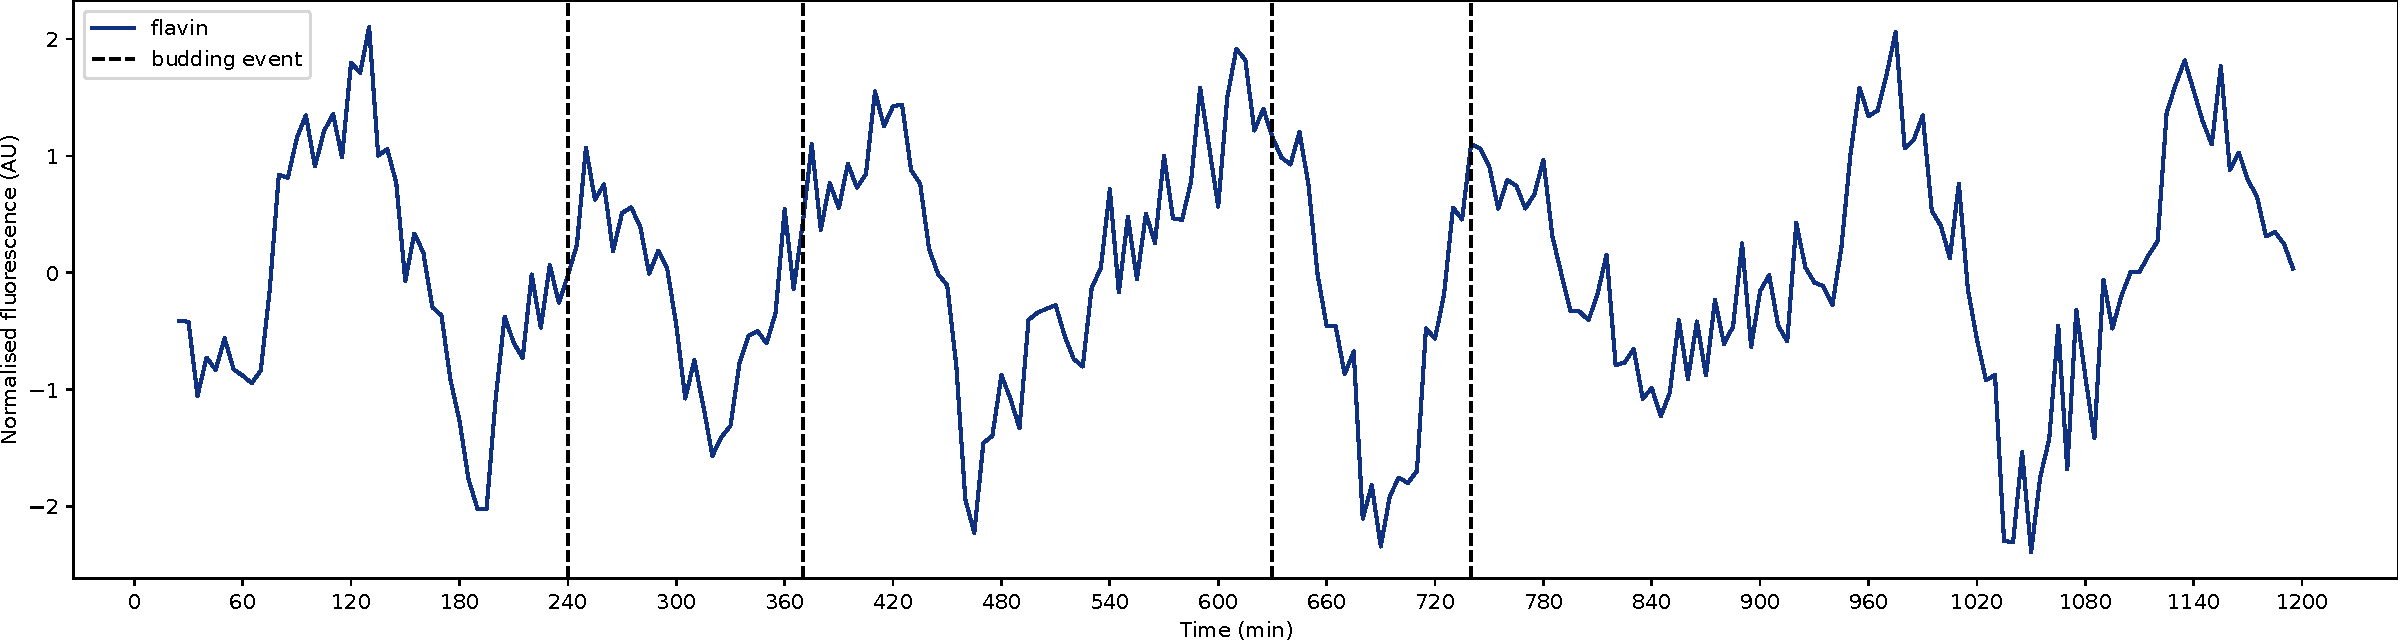
\includegraphics[width=\textwidth]{409_zwf1egf_010-44-1_edit.pdf}
   \caption{
   }
   \label{fig:biology-zwf1-single}
  \end{subfigure}

  \begin{subfigure}[t]{0.45\textwidth}
   \centering
   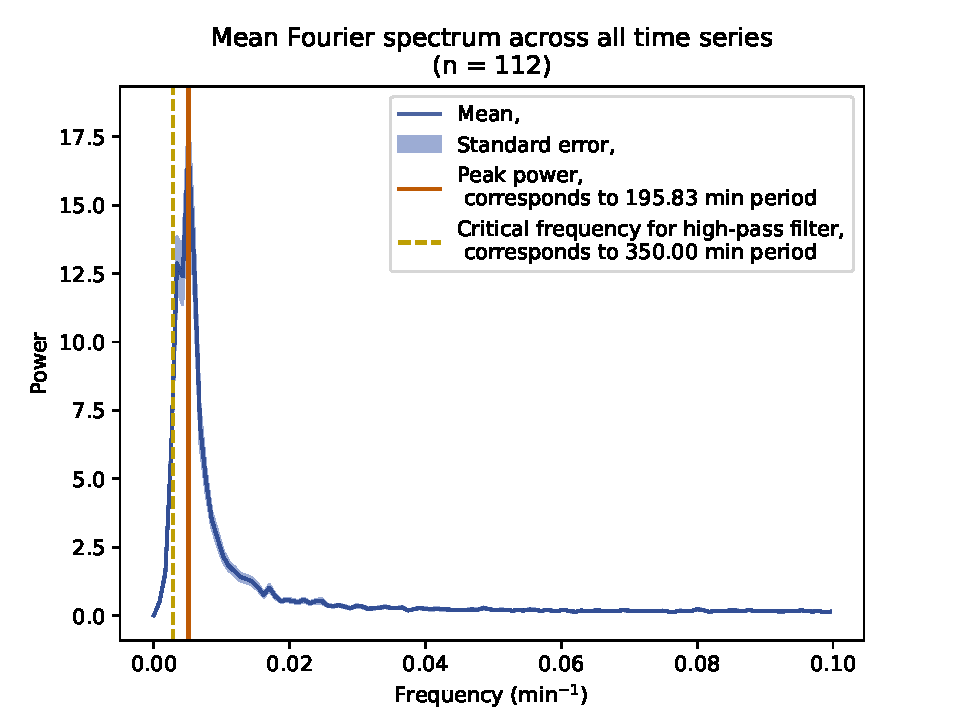
\includegraphics[width=\textwidth]{zwf1egf_409_13.pdf}
   \caption{
   }
   \label{fig:biology-zwf1-fourier}
  \end{subfigure}%
  \begin{subfigure}[t]{0.45\textwidth}
   \centering
   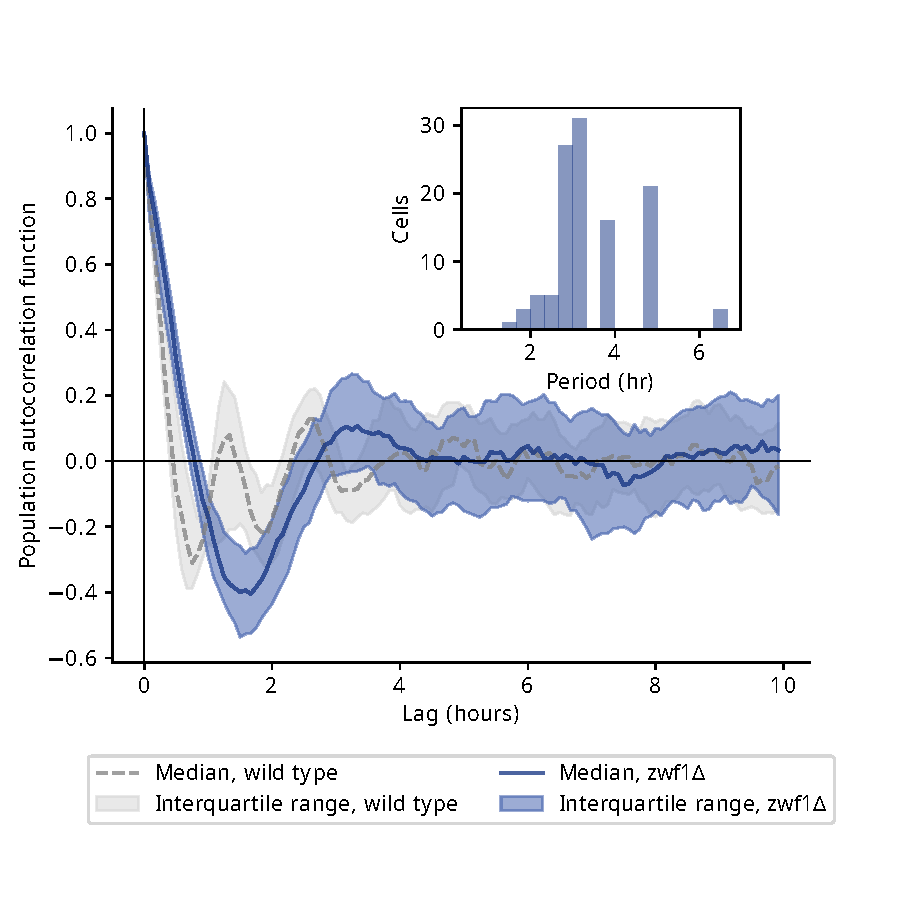
\includegraphics[width=\textwidth]{zwf1egf_409_12.pdf}
   \caption{
   }
   \label{fig:biology-zwf1-acf}
  \end{subfigure}

  \begin{subfigure}[t]{0.45\textwidth}
   \centering
   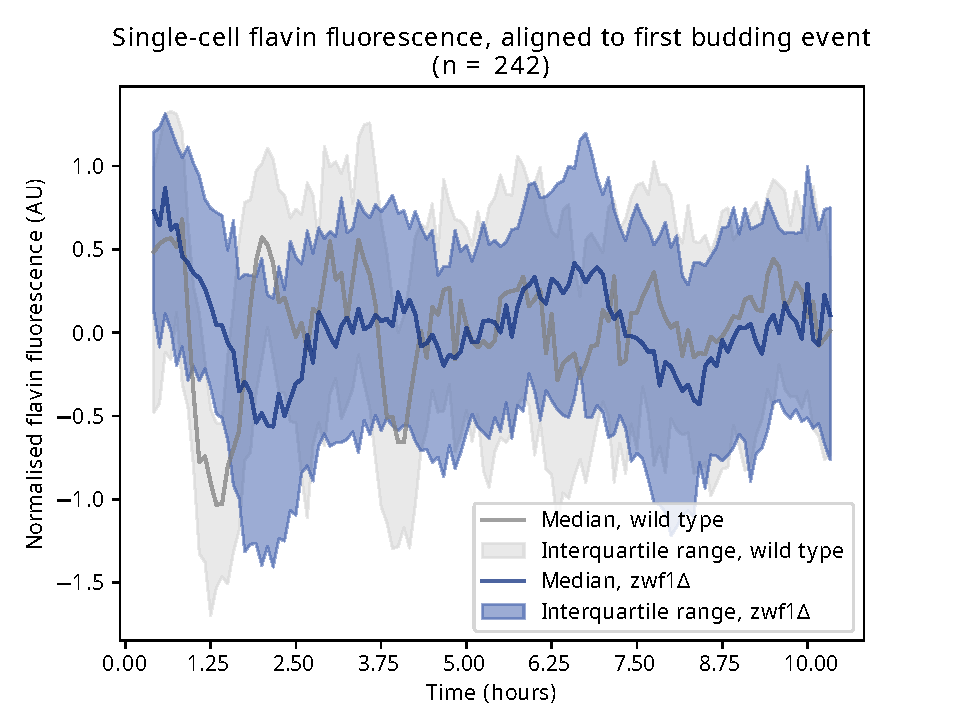
\includegraphics[width=\textwidth]{zwf1egf_409_6.pdf}
   \caption{
   }
   \label{fig:biology-zwf1-median}
  \end{subfigure}%
  \begin{subfigure}[t]{0.45\textwidth}
   \centering
   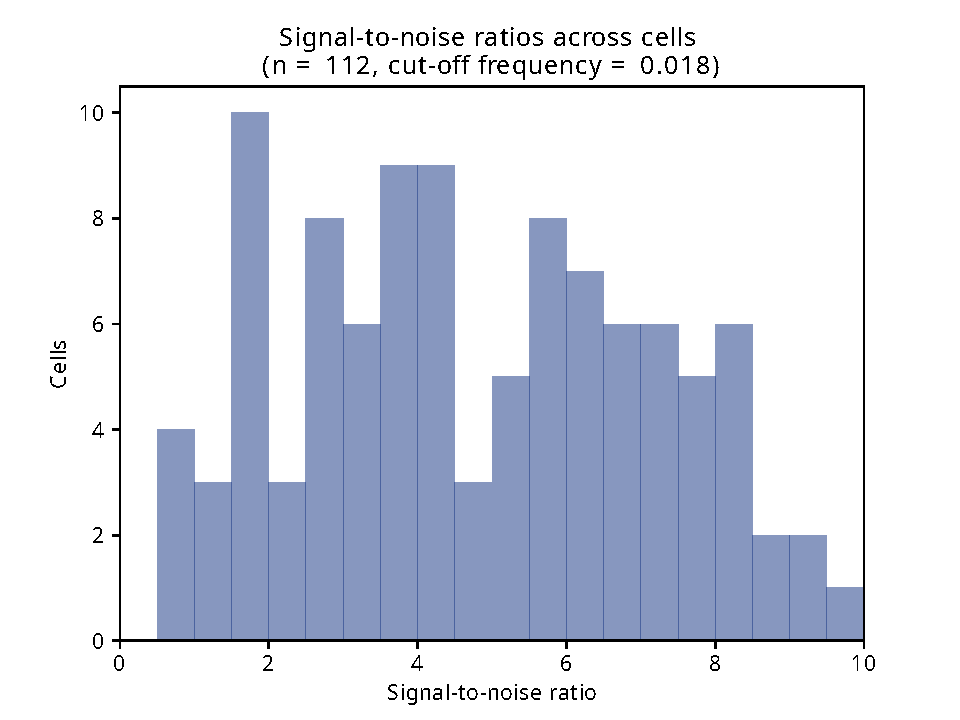
\includegraphics[width=\textwidth]{zwf1egf_409_10.pdf}
   \caption{
   }
   \label{fig:biology-zwf1-snr}
  \end{subfigure}%

  \caption[
    Flavin fluorescence levels in a single, representative \textit{zwf1$\Delta$} cell.
    Mean Fourier spectrum of flavin fluorescence across cells.
    Median autocorrelation function of flavin fluorescence time series, along with the periods across cells.
    Median flavin fluorescence signal across cells, aligned to first budding event.
    Distribution of signal-to-noise ratios of flavin signals from cells.
    Data are from \textit{zwf1$\Delta$} (BY4741) cells in \SI{10}{\gram~\litre^{-1}} glucose.
  ]{
    \textbf{(\ref{fig:biology-zwf1-single})}
    Flavin fluorescence (blue, solid lines) levels in a single, representative \textit{zwf1$\Delta$} cell.
    Vertical lines (black, dashed) indicate budding events.
    \textbf{(\ref{fig:biology-zwf1-fourier})}
    Mean Fourier spectrum of flavin fluorescence across cells.
    \textbf{(\ref{fig:biology-zwf1-acf})}
    Median autocorrelation function of flavin fluorescence time series, along with \textit{\textbf{(inset)}} the periods across cells as determined by the frequency with the greatest power in each signal's Fourier spectrum.
    \textbf{(\ref{fig:biology-zwf1-median})}
    Median flavin fluorescence signal across cells, aligned to first budding event.
    \textbf{(\ref{fig:biology-zwf1-snr})}
    Distribution of signal-to-noise ratios of flavin signals from cells.
    Data are from \textit{zwf1$\Delta$} (BY4741) cells in \SI{10}{\gram~\litre^{-1}} glucose.
  }
  \label{fig:biology-zwf1}
\end{figure}

To investigate whether the \textit{tsa1$\Delta$ tsa2$\Delta$} strain shows metabolic oscillations of a different waveform in single-cell microfluidics, I used a \textit{tsa1$\Delta$ tsa2$\Delta$} strain with the BY4742 background.
Chemostat-based studies suggest that in the \textit{tsa1$\Delta$ tsa2$\Delta$} strain, metabolic cycles are shorter and exhibit an M-shaped dissolved oscillation trace due to an additional dip of oxygen consumption in the reductive-charging phase \parencite{caustonMetabolicCyclesYeast2015}.
% Move to methods?
To be consistent with \textit{zwf1$\Delta$}, cells were pre-cultured and cultured in the same conditions, but with the appropriate supplements for the auxotrophy of BY4742.
%
% Is this because of a wide variety of oscillation frequencies?  Look at the FFT inset, or do additional investigations.

Fig.\ \ref{fig:biology-tsa1tsa2} suggests that the metabolic cycles generated from the auxotrophic \textit{tsa1$\Delta$ tsa2$\Delta$} strain were not consistent, likely due to multiple periods.
Specifically, the Fourier spectra (Fig.\ \ref{fig:biology-tsa1tsa2-fourier}) suggest that \SI{2.45}{\hour} and \SI{3.92}{\hour} oscillations were prominent in the population.
These two prominent periods were obscured by the median fluorescence signal aligned by first budding event (Fig.\ \ref{fig:biology-tsa1tsa2-median}), which merely suggests that a \SI{3}{\hour} oscillation was prominent in the population, and by the median autocorrelation function (Fig.\ \ref{fig:biology-tsa1tsa2-acf}), which suggests that the oscillations were not at a consistent frequency across the population, in contrast to the BY4742 wild-type that showed robust \SI{1.5}{\hour} oscillations.
Fig.\ \ref{fig:biology-tsa1tsa2-snr} additionally shows that the amplitudes and qualities of oscillations were retained, as evidenced by signal-to-noise ratios comparable to the FY4 strain cultured in pyruvate (Fig.\ \ref{fig:biology-compare-snr}).%; ADD STATISTICAL TEST HERE).

\begin{figure}
  \centering
  \begin{subfigure}[t]{1.0\textwidth}
   \centering
   \includegraphics[width=\textwidth]{1649_tsa1tsa2morgan_018-14-1_edit.pdf}
   \caption{
   }
   \label{fig:biology-tsa1tsa2-single}
  \end{subfigure}

  \begin{subfigure}[t]{0.45\textwidth}
   \centering
   \includegraphics[width=\textwidth]{tsa1tsa2morgan_1649_fftrep_freq_edit.pdf}
   \caption{
   }
   \label{fig:biology-tsa1tsa2-fourier}
  \end{subfigure}%
  \begin{subfigure}[t]{0.45\textwidth}
   \centering
   \includegraphics[width=\textwidth]{tsa1tsa2morgan_1649_12.pdf}
   \caption{
   }
   \label{fig:biology-tsa1tsa2-acf}
  \end{subfigure}

  \begin{subfigure}[t]{0.45\textwidth}
   \centering
   \includegraphics[width=\textwidth]{tsa1tsa2morgan_1649_6.pdf}
   \caption{
   }
   \label{fig:biology-tsa1tsa2-median}
  \end{subfigure}%
  \begin{subfigure}[t]{0.45\textwidth}
   \centering
   \includegraphics[width=\textwidth]{tsa1tsa2morgan_1649_10.pdf}
   \caption{
   }
   \label{fig:biology-tsa1tsa2-snr}
  \end{subfigure}

  \caption[
    Flavin fluorescence levels in a single, representative \textit{tsa1$\Delta$ tsa2$\Delta$}cell.
    Overlaid Fourier spectra of flavin fluorescence across cells.
    Median autocorrelation function of flavin fluorescence time series, along with the periods across cells.
    Median flavin fluorescence signal across cells, aligned to first budding event.
    Distribution of signal-to-noise ratios of flavin signals from cells.
    Data are from \textit{tsa1$\Delta$ tsa2$\Delta$} (BY4742) cells in \SI{10}{\gram~\litre^{-1}} glucose.
  ]{
    \textbf{(\ref{fig:biology-tsa1tsa2-single})}
    Flavin fluorescence (blue, solid lines) levels in a single, representative \textit{tsa1$\Delta$ tsa2$\Delta$}cell.
    Vertical lines (black, dashed) indicate budding events.
    \textbf{(\ref{fig:biology-tsa1tsa2-fourier})}
    Overlaid Fourier spectra of flavin fluorescence across cells ($n=212$).
    \textbf{(\ref{fig:biology-tsa1tsa2-acf})}
    Median autocorrelation function of flavin fluorescence time series, along with \textit{\textbf{(inset)}} the periods across cells as determined by the frequency with the greatest power in each signal's Fourier spectrum.
    \textbf{(\ref{fig:biology-tsa1tsa2-median})}
    Median flavin fluorescence signal across cells, aligned to first budding event.
    \textbf{(\ref{fig:biology-tsa1tsa2-snr})}
    Distribution of signal-to-noise ratios of flavin signals from cells.
    Data are from \textit{tsa1$\Delta$ tsa2$\Delta$} (BY4742) cells in \SI{10}{\gram~\litre^{-1}} glucose.
  }
  \label{fig:biology-tsa1tsa2}
\end{figure}

Taken together, there are striking discrepancies between the metabolic cycle observed as dissolved oxygen oscillations from the chemostat and the metabolic cycle observed as flavin autofluorescence oscillations in single-cell conditions in the \textit{zwf1$\Delta$} and \textit{tsa1$\Delta$ tsa2$\Delta$} deletion strains.
These discrepancies warrant further explanation.


\section{Discussion}
\label{sec:biology-discussion}

\subsection{Interpretation of results}
\label{subsec:biology-discussion-interpretation}

This chapter confirms the presence of flavin-based single-cell metabolic cycles, and further confirm that they are autonomous and may gate the cell division cycle across nutrient and genetic perturbations.

My results suggest that yeast cells independently generate the metabolic cycle which locks the cell division cycle in-phase.
This conclusion was supported by the observation that flavin cycles were asynchronous between cells and peaks coincide with bud formation.
These observations were consistent with \textcite{papagiannakisAutonomousMetabolicOscillations2017} and \textcite{baumgartnerFlavinbasedMetabolicCycles2018}.

Results in pyruvate additionally reveal that as the metabolic cycle lengthens, G\textsubscript{1} lengthens but S/M stays the same length, suggesting a model in which a specific phase of the metabolic cycle gates entry into the cell division cycle.
Importantly, metabolic cycles still occurred even when cells did not divide.
This holds true for one-off skipping of cell division and conditions in which cells pause cell division for long periods of time.

My results additionally show that the metabolic cycle and the cell division cycle can be decoupled, reinforcing the idea that the metabolic cycle is autonomous from other cellular oscillators.
In particular, I observed that single-cell flavin oscillations could synchronise and reset phase in response to abrupt starvation, while the cell division cycle was paused.
This observation also suggests that the metabolic cycle is individually generated across cells without the need of a diffusible metabolite as proposed by \textcite{krishnaMinimalPushPull2018}.
The conclusion that the metabolic cycle is generated independently across cells is evidenced by the continued presence of metabolic cycles during starvation even though the cells were physically separated, with nutrient media perfused across them.

The distributions of flavin and mCherry signals during starvation provided some mechanistic basis for the coupling or decoupling between the two oscillators.
This observation suggests that if starvation occurs before START, the cell remains in the G\textsubscript{1} phase.
Otherwise, the cell proceeds through the cell division cycle until it pauses in the G\textsubscript{2} phase.
Such observations strengthen the idea that the metabolic cycle independently gates the early (START) and the late (mitotic exit) phases of the cell division cycle \parencite{ozsezenInferenceHighLevelInteraction2019}.
However, the biochemical mechanism by which the cell uses to reset the phase of its metabolic cycle remains unclear.

My observations confirm that cells adapt their metabolic cycle to nutrient conditions:
the metabolic cycle lengthened when cells were grown on pyruvate, while the cycle exhibited a lengthened period and a lower amplitude when cells were grown on low glucose.
A possible explanation is that nutrient conditions that favour respiration over fermentation --- and thus slower growth rate --- leads to slower YMCs.
% Do the periods conform to those reported by \textcite{papagiannakisAutonomousMetabolicOscillations2017}?  If not, why?

My results suggest discrepancies between chemostat and single-cell studies of the metabolic cycle, in particular, with regards to potassium-deficient conditions and the \textit{zwf1$\Delta$} and \textit{tsa1$\Delta$ tsa2$\Delta$} deletion strains.
Such discrepancies warrant models to explain the observations.
Alternatively, these discrepancies may represent additional cases in which the metabolic cycle is observed in single cells in conditions previously thought to be unfavourable based on chemostat observations, as was the case for metabolic cycles in high-glucose conditions.

I observed that metabolic cycles persist in potassium-deficient conditions, in contrast to \textcite{oneillEukaryoticCellBiology2020} which suggested that the oscillations disappear.
The disappearance of dissolved oxygen cycles can alternatively be explained by a loss of synchrony in the population.
However, while \textcite{oneillEukaryoticCellBiology2020} gradually replaced potassium with sodium over a longer period of time, my experiments included an abrupt potassium depletion but over a shorter period of time.
Therefore, the carbohydrate or amino acid stores that \textcite{oneillEukaryoticCellBiology2020} proposed were responsible for metabolic oscillations may still have been sufficient to drive metabolic oscillations during potassium-deficiency in my experiment.

I also observed that \textit{zwf1$\Delta$} exhibited metabolic cycles, though with varying amplitudes.
This contrasts with \textcite{tuCyclicChangesMetabolic2007}, which suggested that metabolic cycles in this strain were abolished
To reconcile findings, a potential explanation is that cells lose synchrony or the ability to reset phase, while growth is still maintained.
\textit{ZWF1} codes for glucose-6-phosphate dehydrogenase, which catalyses the first step of the pentose phosphate pathway involving the reduction of NADP\textsuperscript{+} to produce NADPH, a key metabolite in the YMC \parencite{nogaeIsolationCharacterizationZWF11990}.
Thus, it is expected that the \textit{zwf1$\Delta$} deletion should affect a broad range of metabolic processes, including flavin oscillations, owing to the role of NAD(P)H redox in the function of the most abundant flavoproteins \parencite{gudipatiFlavoproteomeYeastSaccharomyces2014}.
However, some of the deleterious effects of \textit{zwf1$\Delta$} deletion may be compensated by \textit{ALD6} and \textit{IDP2} as they also catalyse reactions that produce NADPH \parencite{minardSourcesNADPHYeast2005}, therefore, explaining why growth is retained in the \textit{zwf1$\Delta$} strain.

My results additionally suggest that \textit{tsa1$\Delta$ tsa2$\Delta$} exhibits a range of metabolic cycle frequencies.
This observation can be reconciled with the M-shaped dissolved oxygen cycles described by \textcite{caustonMetabolicCyclesYeast2015} through a potential explanation: there are at least two substantial cell populations that each produce a different frequencies of metabolic oscillations, and the changed M-shaped waveform is the sum of the effect of individual cells.
\textit{TSA1} and \textit{TSA2} are paralogous genes that are involved in redox metabolism.
Specifically, these genes code for peroxiredoxins as part of the peroxiredoxin-thioredoxin system, which functions to reduce intracellular reactive oxygen species \parencite{wongCooperationYeastPeroxiredoxins2002}.
In addition, these genes have been suggested to be linked to the circadian rhythm, as evidenced by an approximately \SI{24}{\hour} oscillation in oxidation patterns \parencite{edgarPeroxiredoxinsAreConserved2012}.
Therefore, deletion of these genes may lead to loss of regulation of timekeeping, leading to the different oscillation frequencies.

Taken together, the discrepancies between chemostat and single-cell studies highlight the role of sub-populations that cannot be captured in the chemostat, but possibly in single-cell studies.


\subsection{Study caveats and future directions}
\label{subsec:biology-discussion-caveats}

% Worth reading with the introduction to iron out any logical inconsistencies.

\subsubsection{Characteristics of the single-cell metabolic cycle}
\label{subsec:biology-discussion-caveats-characteristics}

Time series of NAD(P)H oscillations, especially if recorded alongside flavin in the same cells, would strengthen the evidence that flavin autofluorescence oscillations are equivalent to the single-cell metabolic oscillations described by previous microfluidics studies.
%However, due to technical limitations of the fluorescence microscope and image acquisition set-up, I have not been able to acquire such data.
Such data would also provide a novelty: two fluorophores that act as read-outs of the metabolic cycle have, to my knowledge, never been recorded from the same cell.

To explore the link between the components of flavin autofluorescence and cycling of storage lipids as a proposed biochemical mechanism of the metabolic cycle, the \textit{fas1$\Delta$} strain may be studied.
\textit{FAS1} codes for the most abundant flavoprotein, the beta subunit of fatty acid synthetase, which has a role in lipid metabolism \parencite{gudipatiFlavoproteomeYeastSaccharomyces2014}.
The investigation may be strengthened with a rescue experiment using lipid sources such as glycerol trihexanoate or glycerol trioctanoate.
This avenue of exploration may lead to additional insight on the biochemical basis of the yeast metabolic cycle, which is still poorly characterised.

To explore the conditions that make budding yeast cells reset their metabolic cycle phases, future experiments may include adding carbon sources in bulk, using the media-switching system of ALCATRAS.
Such experiments could include acetate, acetaldehyde, or ethanol \parencite{kuangMsn2RegulateExpression2017, krishnaMinimalPushPull2018}.
Insights from such experiments may lead to a broader understanding of the control of the sequence of events in the metabolic cycle.


\subsubsection{Chemostat vs single-cell}
\label{subsec:biology-discussion-caveats-chemostat}

Additional nutrient conditions can be used to address the discrepancies between the chemostat and single-cell microfluidics, namely, low glucose conditions and feast-and-famine conditions.

Low glucose conditions emulate conditions in the chemostat and may lead to long metabolic cycles, thus explaining why cycles with periods up to \SI{14}{\hour} have been observed in chemostats.
However, the glucose concentrations in chemostats are below the tolerance of measurement with current technologies; therefore, I propose that the limiting concentration of \SI{0.010}{\gram~\litre^{-1}} is used.
Experiments with deletion strains can then be performed under these low-glucose conditions to investigate whether such conditions lead to a closer equivalence between chemostat and single-cell studies.

Feast-and-famine conditions have been modelled in chemostat cultivation of yeast \parencite{jonesCyberneticModelGrowth1999}.
Further experiments can therefore use rapid media-switching in ALCATRAS to produce regular glucose pulsing.
In this type of experiment, cells are fed with a glucose-limited medium for an amount of time, then switched on to a glucose-rich medium for a short period of time (approximately \SI{10}{\minute}), and the cycle repeats.
The interval between glucose pulses can be varied to investigate the effect of an external entraining mechanism on the system of coupled oscillators that defines the yeast metabolic cycle.
This design would be similar to \textcite{charvinForcedPeriodicExpression2009}, which investigated the effect of intervals of glucose pulsing on the cell division and circadian cycles in budding yeast.
A glucose pulsing experiment can thus also lead to a mathematical model of coupled oscillations in the yeast metabolic cycle.
